\documentclass[aspectratio=169, 9pt,t]{beamer}
\graphicspath{{figures/}} % Setting the graphicspath

% Theme settings
\usetheme{Madrid}
\usecolortheme{default}
\setbeamertemplate{navigation symbols}{}   % removes navigation symbols such as 'next page'
\setbeamertemplate{footline}{}             % remove line with name, date, page nr.
\setbeamercolor*{frametitle}{bg=white}     % remove background from frametitle
\usepackage{caption}
% \captionsetup[figure]{labelformat=empty}% redefines the caption setup of the figures environment in the beamer class.
\setbeamersize{text margin left=20pt,text margin right=10pt}
\usefonttheme[onlymath]{serif} % makes beamer math look like article math
\usepackage{hyperref}

%======================= title page info =======================
\title{Recent progress in global PDF determination and the path to N3LO}
\subtitle{\small Based on 2401.08749 (NNPDF4.0 QED), 2401.10319 (NNPDF4.0 MHOU), and 2402.18635 (NNPDF4.0 aN3LO)}
\date{Joint Northern UK Journal Club  \\[0.1cm] 23 April 2024}
\author{Roy Stegeman}
\institute{\small The University of Edinburgh}


%======================= page numbering =======================
\addtobeamertemplate{navigation symbols}{}{ \usebeamerfont{footline}
  \insertframenumber / \inserttotalframenumber \hspace*{2mm} \\ \vspace*{1mm}
}


%=================================== colors ====================================
\definecolor{RoyBlue}{RGB}{22, 46, 69}
\definecolor{RoyGrey}{RGB}{64, 88, 128}

\newcommand{\hlme}[1]{{\color{red}\bf #1}} % highlight me

\setbeamercolor{structure}{fg=RoyBlue} % itemize, enumerate, etc
\setbeamercolor{frametitle}{fg=RoyGrey}
\setbeamercolor{section in head/foot}{bg=RoyBlue}


%======================= add progress dots to headline =========================
% \setbeamertemplate{headline}{%
%     \begin{beamercolorbox}[ht=4mm,dp=4mm]{section in head/foot}
%         \insertnavigation{\paperwidth}
%     \end{beamercolorbox}%
% }%
% \makeatother


%======================= add section title page ================================
\AtBeginSection[]{
  \begin{frame}
  \vfill
  \centering
    \usebeamerfont{title}\insertsection\par%
  \vfill
  \end{frame}
}


%=================================== titlepage =================================
\titlegraphic{\vspace*{6mm}
  
\includegraphics[height=1.5cm]{logos/edi_logo.png} \hspace{10mm}
  % 
\includegraphics[height=0.8cm]{logos/nnpdf_logo_official.pdf} \hspace{10mm}
  
\includegraphics[height=1.5cm]{logos/higgs_logo.jpg}
}

\defbeamertemplate{title page}{noinstitute}[1][]
{
  \vbox{}
  \vfill
  \begingroup
    \centering
    \begin{beamercolorbox}[sep=8pt,center,#1]{title}
      \usebeamerfont{title}\inserttitle\par%
      \ifx\insertsubtitle\@empty%
      \else%
        \vskip0.25em%
        {\usebeamerfont{subtitle}\usebeamercolor[fg]{subtitle}\insertsubtitle\par}%
      \fi%
    \end{beamercolorbox}%
    \vskip2em\par
    \begin{beamercolorbox}[sep=0pt,center,#1]{author}
      \usebeamerfont{author}\insertauthor
    \end{beamercolorbox}
  \begin{beamercolorbox}[sep=0pt,center,#1]{author}
    \usebeamerfont{institute}\insertinstitute
  \end{beamercolorbox}
  \vspace*{8pt}
  \vspace*{16pt}
    \begin{beamercolorbox}[sep=0pt,center,#1]{date}
      \usebeamerfont{date}\insertdate
    \end{beamercolorbox}\vskip0.5em
    {\usebeamercolor[fg]{titlegraphic}\inserttitlegraphic\par}
  \endgroup
  \vfill
}

\makeatletter
\setbeamertemplate{title page}[noinstitute][colsep=-4bp,rounded=true,shadow=\beamer@themerounded@shadow]
\makeatother


\begin{document}
{
\setbeamertemplate{headline}{} % remove headline from titlepage
\begin{frame}
  \titlepage
\end{frame}
}

\setbeamertemplate{enumerate items}[default]

\pgfdeclarelayer{bg}    % declare background layer
\pgfsetlayers{bg,main}  % set the order of the layers (main is the standard layer)


% SLIDES =======================================================================
\newcommand{\nn}{\vspace*{1em}}


% \begin{frame}{Introduce NNPDF}
% \end{frame}



\begin{frame}{Motivation}
  $$\sigma(x,Q^2)=\sum_i \int_x^1 \frac{dz}{z} \mathcal{L}_{ij}(z,\mu^2)\hat{\sigma}_{ij}\left(\frac{x}{z},\frac{Q^2}{\mu^2},\alpha_s\right)$$

  \begin{columns}
    \begin{column}{0.49\textwidth}
      \begin{itemize}
        \item Predictions for collider processes rely on PDFs and matrix elements
        \item PDF uncertainties often the dominant source of uncertainty
        \item Current standard in PDF fits is NNLO in QCD
      \end{itemize}

      \vspace*{0.5em}
      Progress towards the next generation of PDFs:
      \begin{itemize}
        \item QED effects
        \item (approximate) N3LO
        \item Accounting for missing higher order uncertainties
      \end{itemize}
    \end{column}
    \begin{column}{0.49\textwidth}
      \begin{figure}
        \centering
        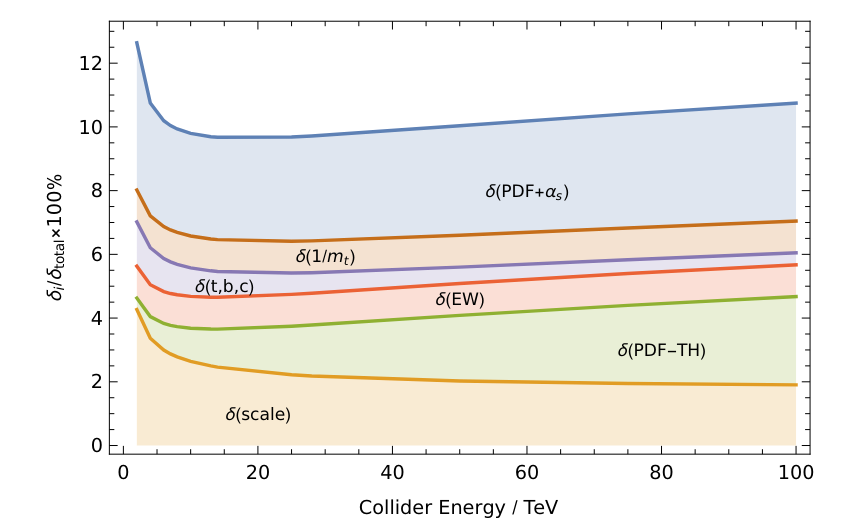
\includegraphics[width=0.8\textwidth]{figures/sources_of_unc_higgs.png}
        \caption*{ \small Uncertainties for inclusive Higgs production \\  {\color{gray}\small [Dulat, Lazopoulos, Mistleberger: 1802.00827]}}
      \end{figure}
    \end{column}
  \end{columns}
\end{frame}


% \begin{frame}{Motivation}
%   PDFs, along with $\alpha_s$, are often a dominant source of uncertainty for predictions of LHC cross-sections
%   \begin{columns}
%     \begin{column}{0.49\textwidth}
%       \vspace*{1em}

%       Requirements for the next generation of PDFs are threefold:
%       \begin{itemize}
%         \item To exploit the impressive progress in N3LO calculations we require PDFs of the same order
%         \item Missing higher order uncertainties (MHOUs) for some observables are larger than the experimental uncertainty and can thus no longer be neglected
%         \item The level of precision aimed for at the LHC no longer allows neglecting EW corrections
%       \end{itemize}

%       \vspace*{1em}
%       Focus on QED, but first briefly mention N3LO and MHOU
%     \end{column}

%     \begin{column}{0.49\textwidth}
%       \begin{figure}
%         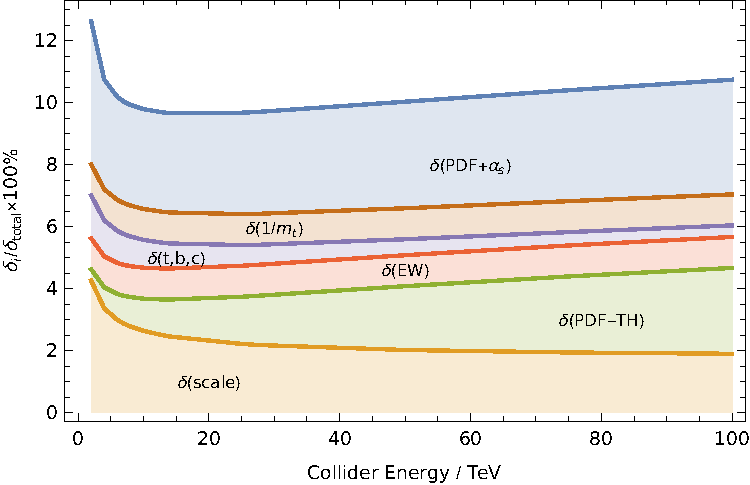
\includegraphics[width=0.8\textwidth]{figures/sources_of_unceratinty.pdf}
%         \caption*{Uncertainties for inclusive Higgs production \\
%         \color{gray}\small [HL-LHC: 1902.00134]}
%       \end{figure}
%     \end{column}
%   \end{columns}
% \end{frame}




\section{QED effects in PDFs}

\begin{frame}{Including QED corrections in a PDF set}
  The current standard for PDFs determination is at NNLO in QCD, however  $\alpha(M_z) \sim \alpha_s^2(M_Z)$

  \begin{columns}
    \begin{column}{0.49\textwidth}

      \vspace*{1em}
      Including QED corrections in PDFs consists of \vspace*{0.5em}
      \begin{itemize}
        \item QED corrections to DGLAP (at $\mathcal{O}(\alpha)$, $\mathcal{O}(\alpha \alpha_s)$ and $\mathcal{O}(\alpha^2))$: \\
        $P_{QED}=\alpha P_{ij}^{(0,1)}+\alpha \alpha_s P_{ij}^{(1,1)}+\alpha^2 P_{ij}^{(0,2)}+\ldots$
        \vspace*{0.5em}
        \item Adding a photon PDF and including photon initiated contributions to cross-sections \\
        The momenum sumrule is modified accordingly:
        \begin{equation*}
          \int_0^1 dx\, \left(  x\Sigma(x,Q^2) + xg(x,Q^2) + x\gamma(x,Q^2) \right) =1
        \end{equation*}
      \end{itemize}
    \end{column}

    \begin{column}{0.49\textwidth}
      \begin{figure}
        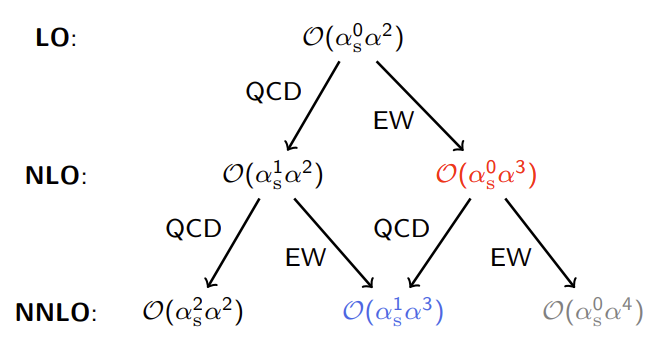
\includegraphics[width=0.99\textwidth]{figures/ewcorrections_dy.png}
        \caption*{Example: EW corrections in DY\\ {\color{gray}\small [C. Schwan DIS 2021]}}
      \end{figure}
    \end{column}
  \end{columns}
\end{frame}


\begin{frame}{Determination of the photon PDF}
  \begin{columns}[T]
    \begin{column}{0.59\textwidth}
      Initially the photon PDF has been determined in different ways:
      \begin{itemize}
        \item physical model: sensitive to underlying model
        \item fitting: data does not provide strong constraints
      \end{itemize}

      \vspace*{0.5em}
      However with the LUXqed approach it can be computed perturbatively \\
      based on the observation that the heavy-lepton production cross-section can be written in two ways:
      \begin{itemize}
        \item in terms of structure functions $F_2$, $F_L$
        \item in terms of PDFs (including the photon)
      \end{itemize}

      \vspace*{0.5em}
      luxQED result {\color{gray}\small[Manohar, Nason, Salam, Zanderighi: 1607.04266, 1708.01256]}:
      \vspace*{-0.8em}
      \begin{equation*}
        \begin{split}
          & x \gamma(x, \mu^2)
          =
          \frac{2}{\alpha (\mu^2)} \int\limits_x^1 \frac{dz}{z}
          \Biggl\{ \int_{m_p^2x^2 \over 1-z}^{\mu^2 \over 1-z} \frac{dQ^2}{Q^2}
          \alpha^2(Q^2) \Biggl[ -z^2 F_L(x/z, Q^2) \\
          & + \left( z P_{\gamma q}(z) + \frac{2 x^2 m_p^2}{Q^2} \right)
          F_2(x/z, Q^2)\Biggr] - \alpha^2(\mu^2) z^2 F_2(x/z, \mu^2)\Biggr\}
        \end{split}
      \end{equation*}
    \end{column}

    \begin{column}{0.39\textwidth}
      \vspace*{-2.5em}
      \begin{figure}
        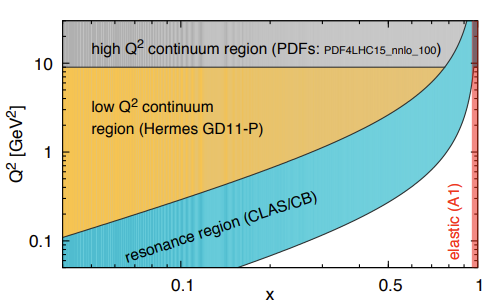
\includegraphics[width=0.89\textwidth]{figures/dataluxqed.png}
        \caption*{Input to construct $F_2$ and $F_L$}
        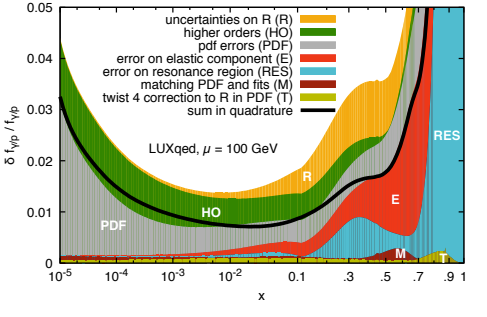
\includegraphics[width=0.89\textwidth]{figures/luxQED_uncs.png}
        \caption*{Sources of uncertainty}
      \end{figure}
    \end{column}
  \end{columns}
\end{frame}


\begin{frame}{LUXqed PDF determinations}
  LUXqed has been used in all of the most recent QED PDFs:
  \begin{itemize}
      \item LUXqed\_plus\_PDF4LHC15 {\color{gray}\small [1607.04266]}
      \item LUXqed17\_plus\_PDF4LHC15 {\color{gray}\small [1708.01256]}
      \item MMHT2015qed {\color{gray}\small [1907.02750]}
      \item NNPDF3.1luxQED {\color{gray}\small [1712.07053]}
      \item CT18lux and CT18qed {\color{gray}\small [2106.10299]}
      \item MSHT20QED {\color{gray}\small [2111.05357]}
      \item MSHT20qed\_an3lo {\color{gray}\small [2312.07665]}
      \item NNPDF4.0QED {\color{gray}\small [2401.08749 ]}
  \end{itemize}
\end{frame}

\begin{frame}{The photon PDF}
  \begin{columns}[T]
    \begin{column}{0.59\textwidth}
      An iterative procedure  is used to address the interplay between the photon and other PDFs due to the momentum sumrule
      \begin{equation*}
        \int_0^1 dx\, \left(  x\Sigma(x,Q^2) + xg(x,Q^2) + x\gamma(x,Q^2) \right) =1
      \end{equation*}
    \end{column}

    \begin{column}{0.39\textwidth}
      \vspace*{-1.5em}
      \begin{figure}
        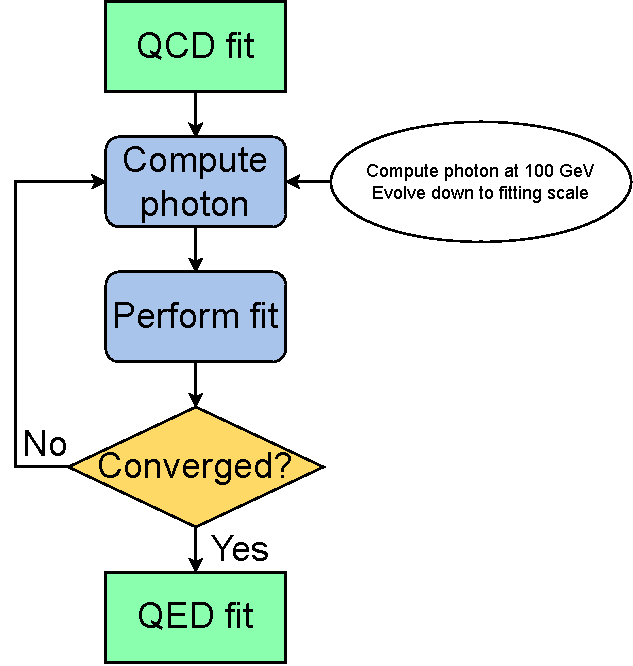
\includegraphics[width=0.9\textwidth]{figures/luxqed_iteration.pdf}
        \caption*{\color{gray}\small [NNPDF3.1QED: 1712.07053]}
      \end{figure}
    \end{column}
  \end{columns}

\end{frame}


\begin{frame}{Results: Impact of the photon on other PDFs}

  \begin{figure}[!t]
    \centering
    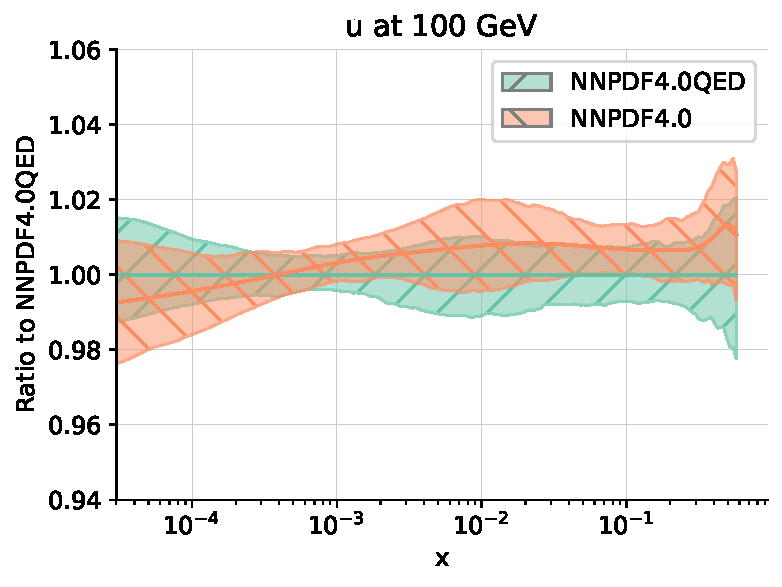
\includegraphics[width=.49\textwidth]{figures/plot_pdfs_u_qed.pdf}
    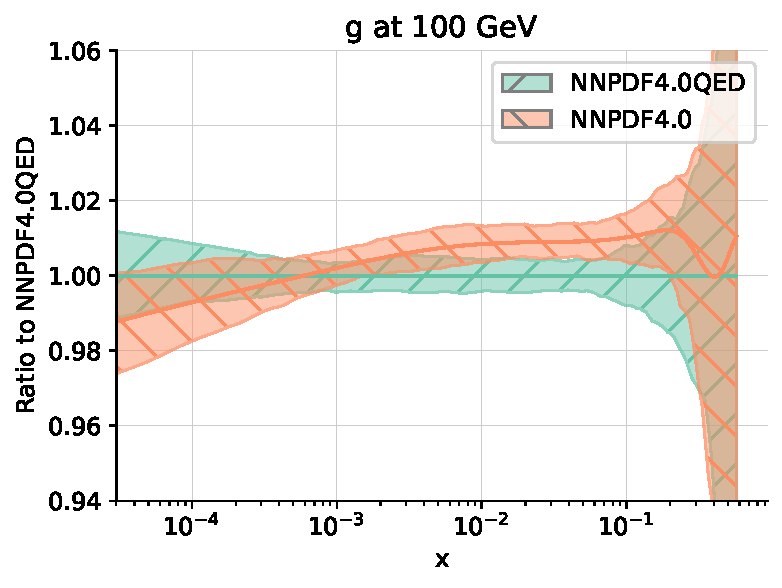
\includegraphics[width=.49\textwidth]{figures/plot_pdfs_g_qed.pdf}\\
  \end{figure}

  \begin{itemize}
    \item Non-negligible impact, but PDFs are in agreement within uncertainty
    \item Gluon reduced due to momentum sum rule with photon carrying additional momentum
  \end{itemize}
\end{frame}


% \begin{frame}{Results: photon PDF and luminosity}
%   \begin{center}
%     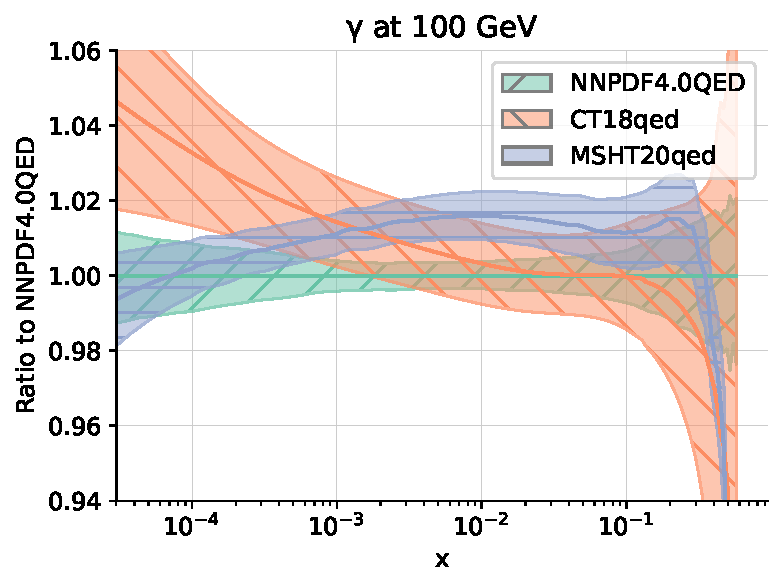
\includegraphics[width=0.3\textwidth]{figures/photon_comparison.pdf}
%     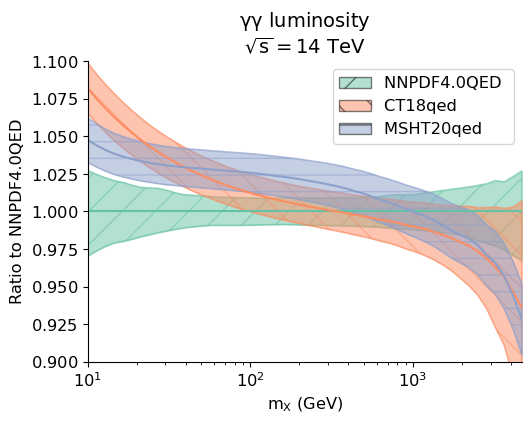
\includegraphics[width=0.3\textwidth]{figures/pp_lumi_comparison.png}
%     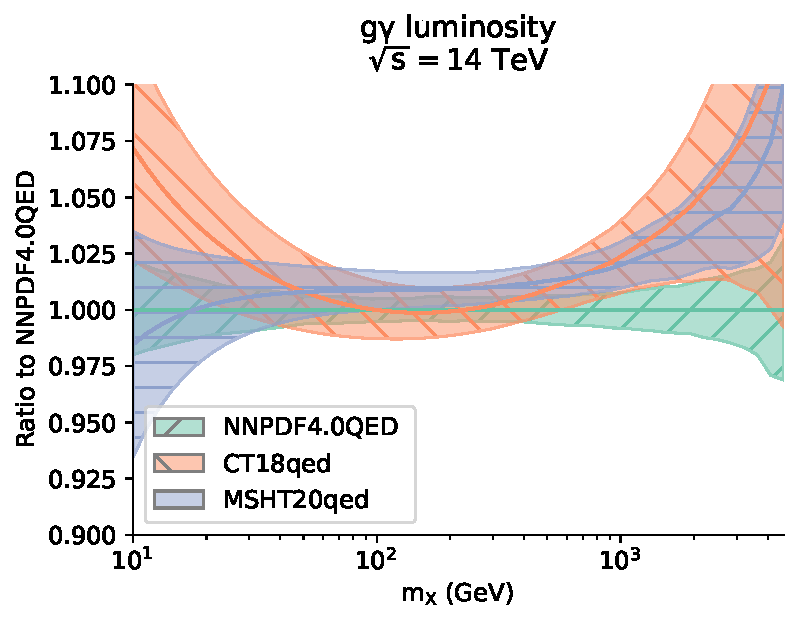
\includegraphics[width=0.3\textwidth]{figures/gp_lumi_comparison.pdf}
%   \end{center}
%   \begin{itemize}
%     \item Because all groups use the luxQED formalism, the photon PDFs agree at percent level
%     \item Luminosity generally in agreement, but differ at very small and very large invariant mass
%   \end{itemize}
% \end{frame}


\begin{frame}{Results: phenomenological impact}
  \begin{columns}[T]
    \begin{column}{0.49\textwidth}
      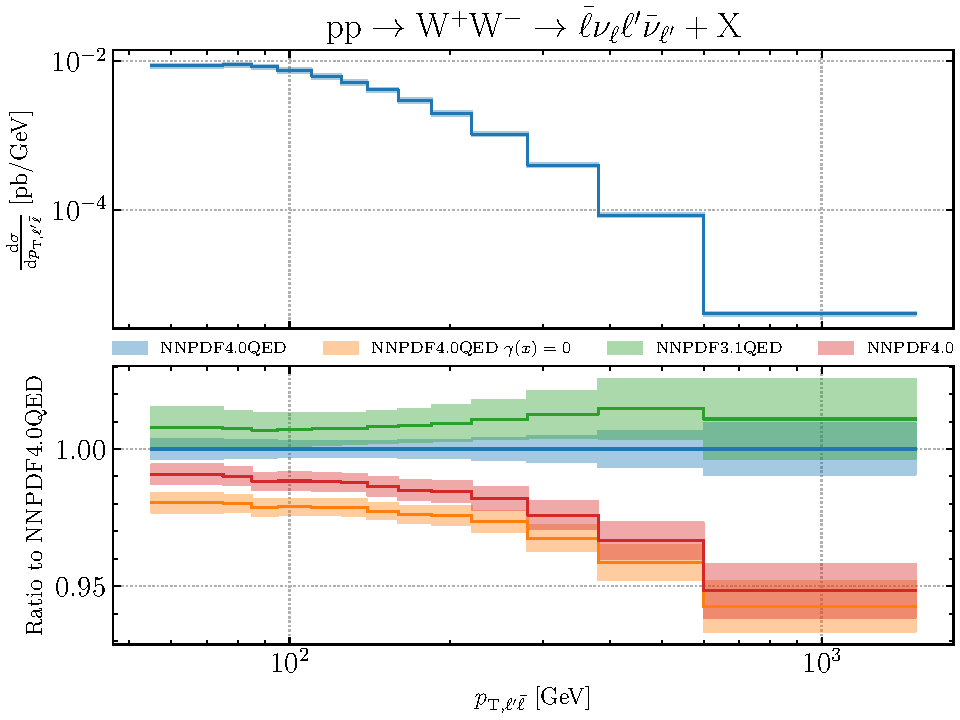
\includegraphics[width=0.9\textwidth]{figures/NNPDF_WPWM_14TEV_40_PHENO-internal.pdf}
    \end{column}
    \begin{column}{0.49\textwidth}
      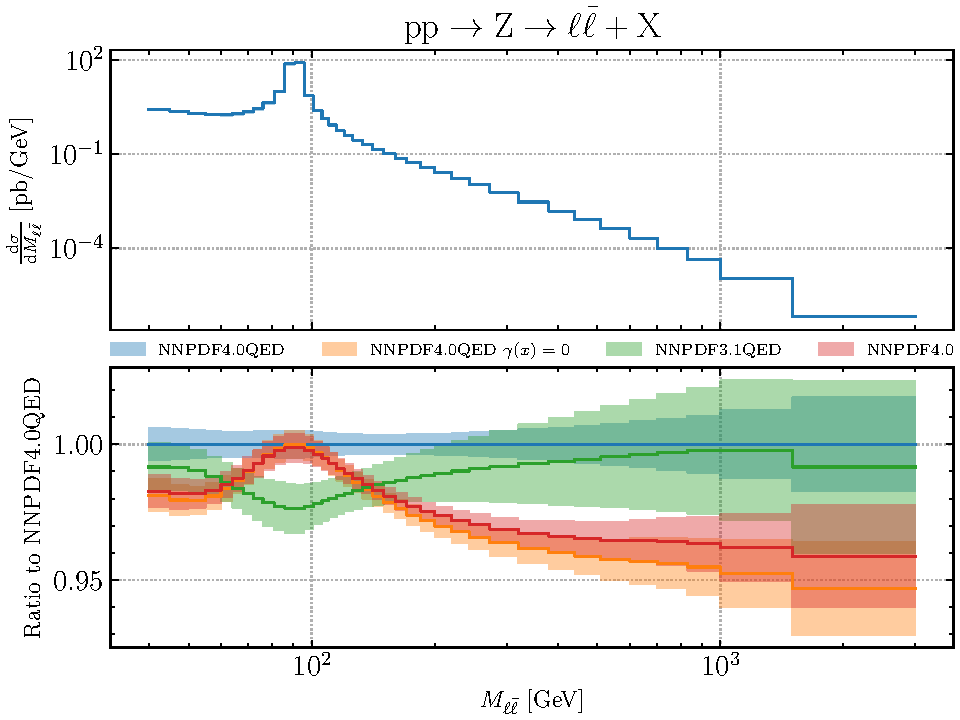
\includegraphics[width=0.9\textwidth]{figures/NNPDF_DY_14TEV_40_PHENO-internal.pdf}
    \end{column}
  \end{columns}

  \vspace*{1em}
  \begin{itemize}
    \item Here photon initiated contributions are included
    \item Non-negligable QED corrections in the large invariant mass and large-$p_T$ regions relevant for new physics searches
    \item Negligible impact around the $Z$-peak
  \end{itemize}
\end{frame}



% ============================================================================
\section{Theory in puts for approximate N3LO PDFs}

\begin{frame}{Theory requirements for PDFs at N3LO}
  Several theory inputs are needed in a PDF fit:
  \begin{itemize}
    \item Splitting functions for DGLAP evolution \\

    \item Matching conditions for heavy-quark mass schemes \\
    $ f_i^{\left(n_f+1\right)}\left(x, Q^2\right)=A_{i j}\left(x, \alpha_s\right) f_j^{\left(n_f\right)}\left(x, Q^2\right) $
    \item DIS coefficient functions
    \item Hadronic cross sections,
  \end{itemize}

  \vspace*{1em}
  Not all available at N3LO, but information is available for all. What is the best we can do?
  \begin{itemize}
    \item Use N3LO calculations where known
    \item Construct approximate results where possible
    \item Account for theory uncertainties of the missing or incomplete higher order
  \end{itemize}

  \vspace*{0.5em}
  No need to wait for complete N3LO results and more information can be included as it becomes available
\end{frame}


\begin{frame}{Splitting functions}
  Complete results for the N3LO splitting functions are not yet available, but a lot of information exists (with important contributions from Liverpool and Edinburgh):
  \begin{itemize}
    \item Singlet and non-singlet Mellin moments
    {\color{gray}\small [Davies, Falcioni, Herzog, Kom, Moch, Ruijl, Ueda, Vermaseren, Vogt: 1707.08315, 1610.07477, 2202.10362, 2111.15561, 2302.07593, 2307.04158]}
    \item Large-$n_f$ limit {\color{gray}\small [Davies, Vogt, Ruijl, Ueda, Vermaseren: 1610.0744]}
    \item Small-x limits (BFKL resummation) {\color{gray}\small [Bonvini and Marzani: 1805.06460] [Davies, Kom, Moch, Vogt: 2202.10362]}
    \item Large-x limits (threshold resummation) {\color{gray}\small [Duhr, Mistlberger, Vita 2205.04493], [Henn, Korchemsky, Mistlberger: 1911.10174], [Soar, Moch, Vermaseren, Vogt: 0912.0369]}
  \end{itemize}

  \vspace*{2em}
  \begin{center}
    How can we use this information to construct approximate splitting functions?
  \end{center}

\end{frame}


\begin{frame}{Splitting functions}

  The approximation is performed in Mellin space as an expansion in $nf$, where any double counting terms present in the resummed small-$x$ and large-$x$ expressions are removed

  $$\gamma_{i j}^{(3)}=\gamma_{i j, n_f}^{(3)}+\gamma_{i j, N \rightarrow \infty}^{(3)}+\gamma_{i j, N \rightarrow 0}^{(3)}+\gamma_{i j, N \rightarrow 1}^{(3)}+\widetilde{\gamma}_{i j}^{(3)}$$

  \vspace*{1em}
  The remainder term $\widetilde{\gamma}_{i j}^{(3)}$ is constructed as a linear combination of interpolating functions:
  \begin{itemize}
    \item A function for the leading unknown large-N contribution
    \item A function for the two leading unknown small-N contribution
    \item Functions for the subleading small-N and large-N contributions
  \end{itemize}

  \vspace*{0.5em}
  Then, vary the subleading contributions included in the basis of interpolating functions to estimate "incomplete higher order uncertainties" (IHOU) on the splitting functions

  \vspace*{1em}
  More details on how to account for IHOUs in a fit follows later
\end{frame}


\begin{frame}{Splitting functions}
  \begin{figure}
    \centering
    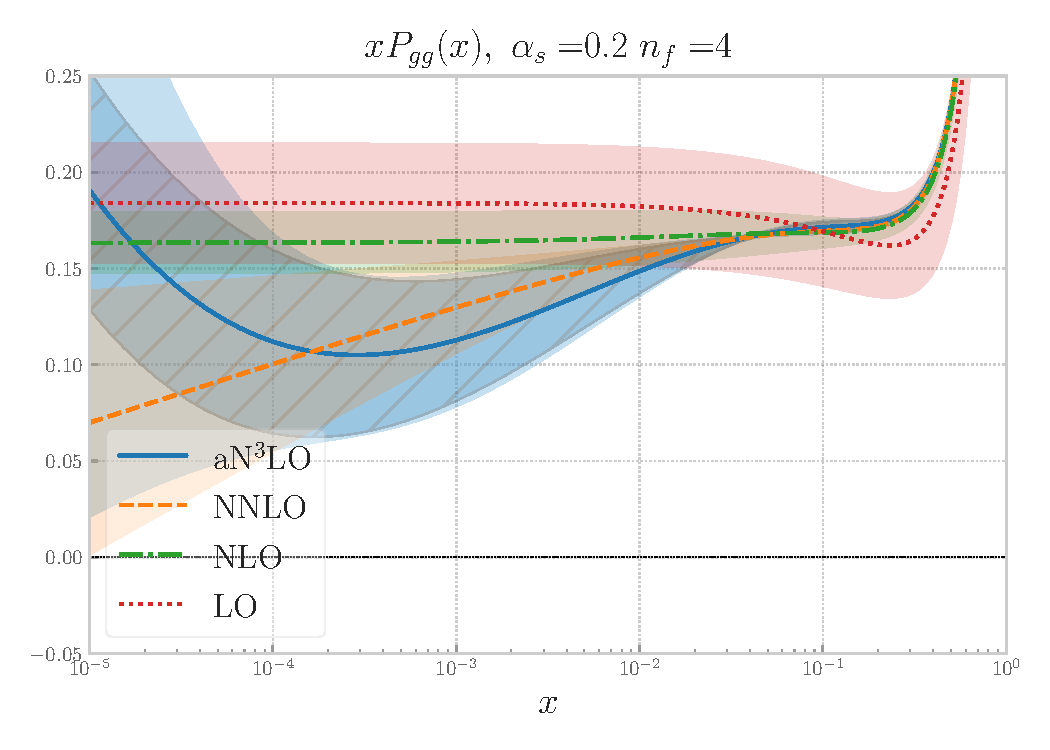
\includegraphics[width=.4\textwidth]{figures/gamma_gg_totu_logx.pdf}
    % 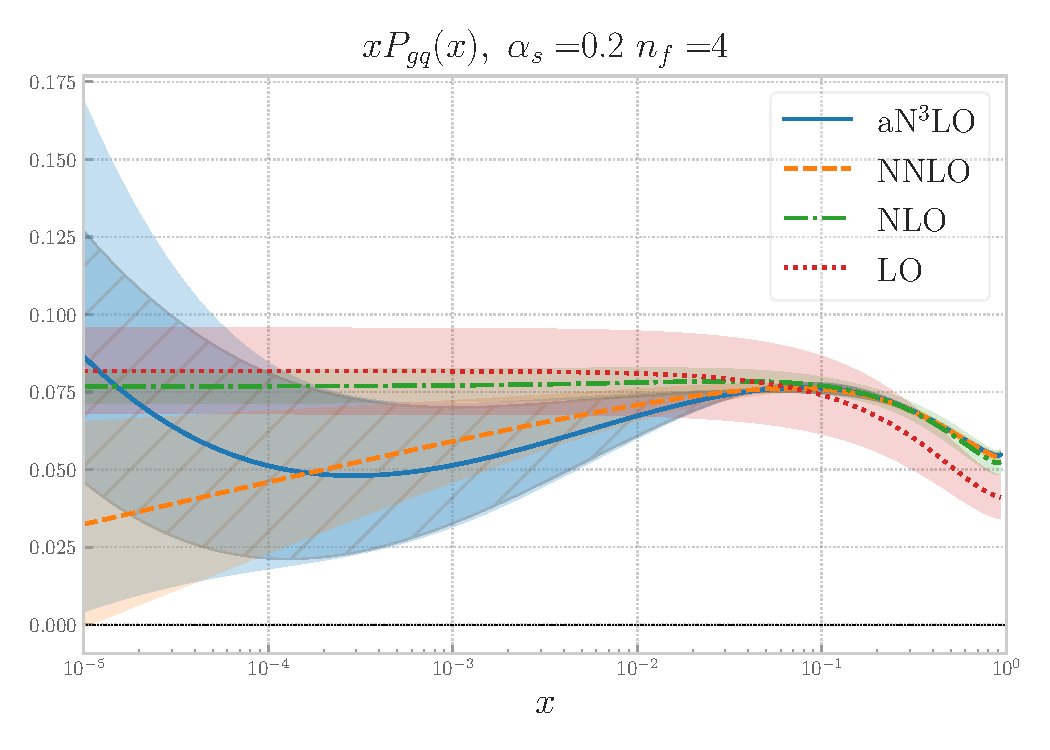
\includegraphics[width=.4\textwidth]{figures/gamma_gq_totu_logx.pdf} \\
    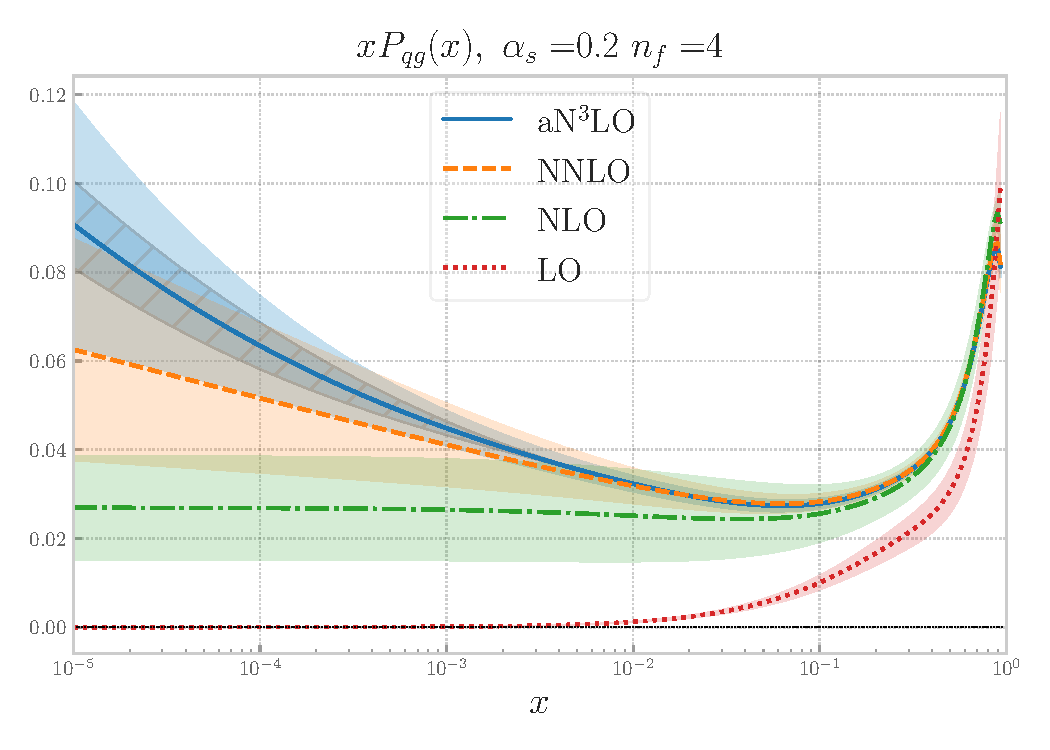
\includegraphics[width=.4\textwidth]{figures/gamma_qg_totu_logx.pdf}
    % 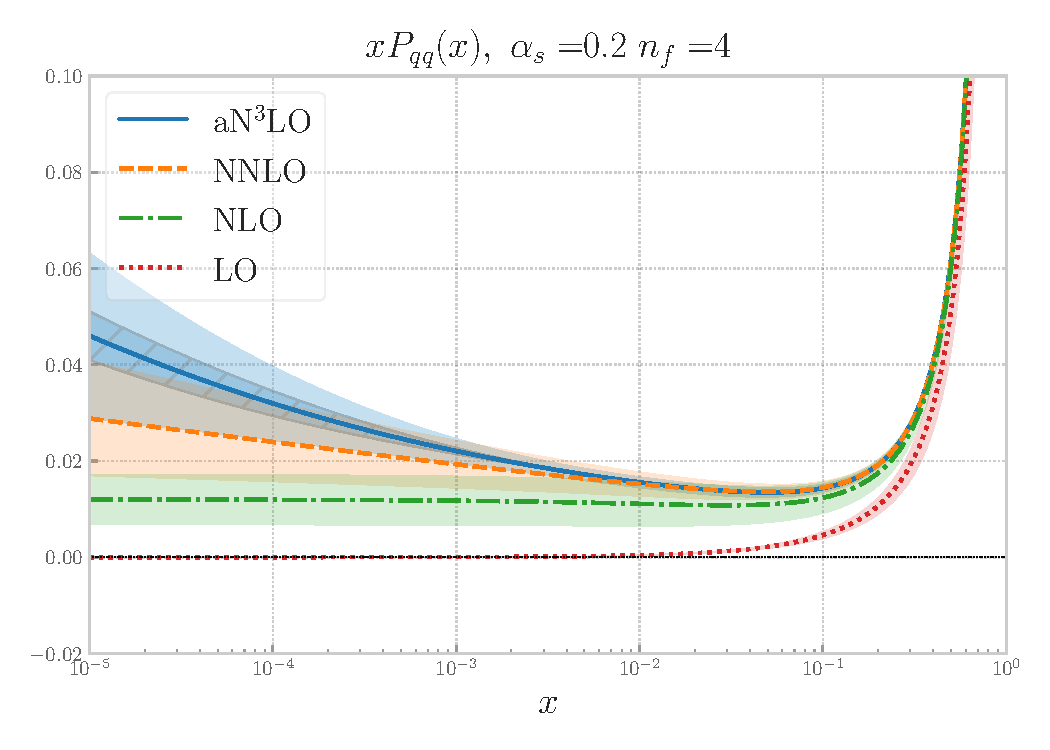
\includegraphics[width=.4\textwidth]{figures/gamma_qq_totu_logx.pdf}
  \end{figure}
  \begin{itemize}
    \item Shown uncertainties are estimated missing higher order uncertainty (MHOU) through factorization scale variations. Light blue is sum in quadrature of MHOU and IHOU
    \item Good perturbative agreement at large-$x$
    \item IHOU are not negligible
  \end{itemize}
\end{frame}



\begin{frame}{DGLAP evolution}
  NNPDF4.0 evolved from $Q=1.65$ GeV to $Q=100$ GeV

  \begin{columns}
    \begin{column}{0.59\textwidth}
      \begin{figure}[!t]
        \centering
        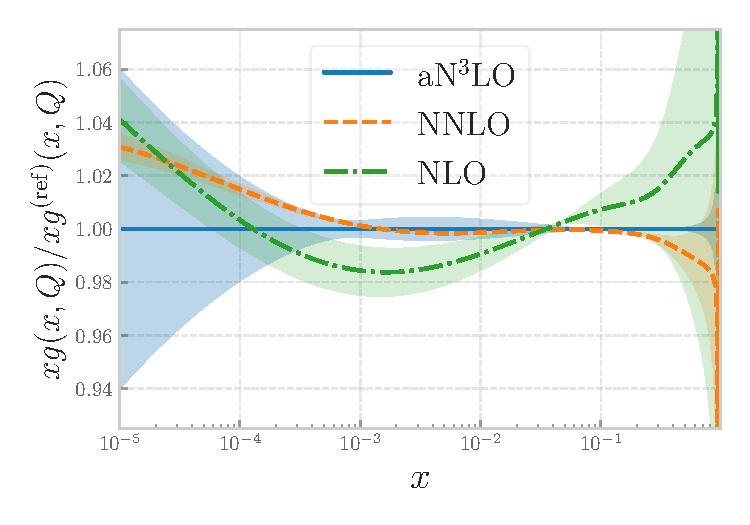
\includegraphics[width=0.49\textwidth]{figures/N3LOevolution-q100gev-ratios_expanded_0.pdf}
        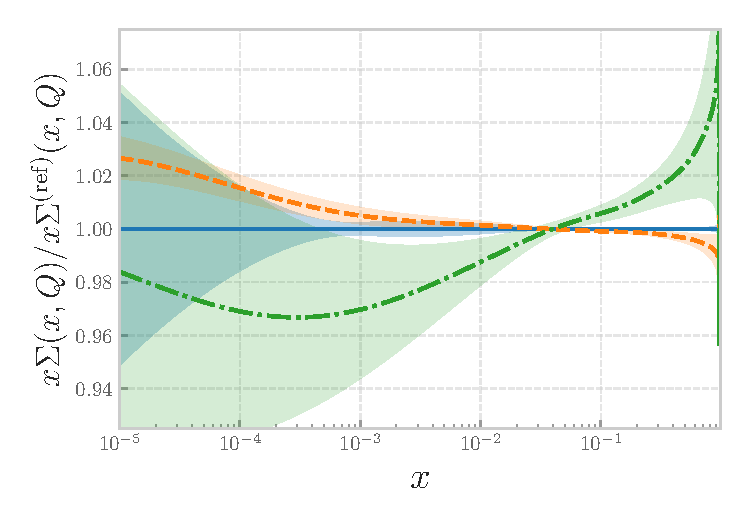
\includegraphics[width=0.49\textwidth]{figures/N3LOevolution-q100gev-ratios_expanded_1.pdf}\\
        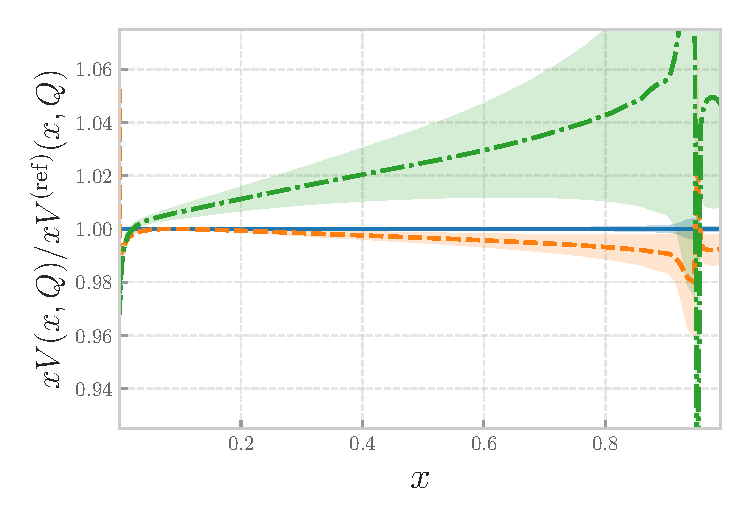
\includegraphics[width=0.49\textwidth]{figures/N3LOevolution-q100gev-ratios_expanded_2.pdf}
        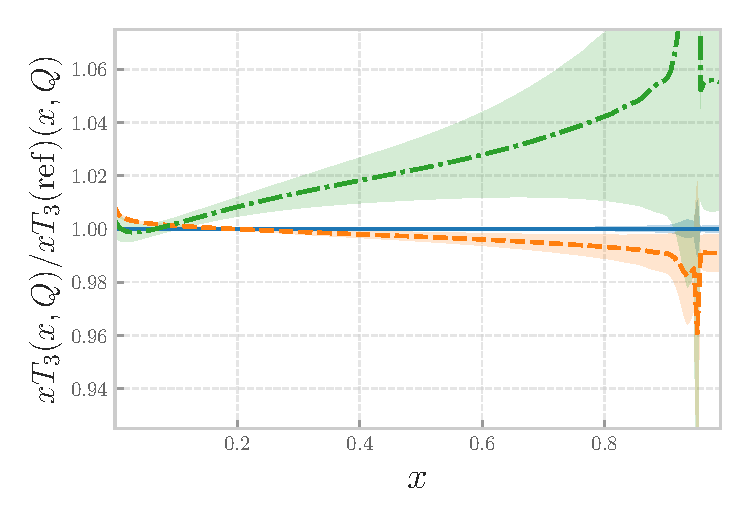
\includegraphics[width=0.49\textwidth]{figures/N3LOevolution-q100gev-ratios_expanded_3.pdf}
      \end{figure}
    \end{column}
    \begin{column}{0.39\textwidth}
      \begin{itemize}
        \item Effects of N3LO corrections to DGLAP evolution at most percent level, except at small-$x$ and large-$x$
        \item Good perturbative convergence
      \end{itemize}
    \end{column}
  \end{columns}
\end{frame}

\begin{frame}{DIS coefficient functions}
  \begin{itemize}
    \item DIS coefficient functions are known up to N3LO in the massless limit (again with contributions from Liverpool)
    \item Massive coefficient functions can be constructed as a linear combination of the known limits ($Q^2 \rightarrow m_h^2$, $Q^2\gg m_h^2$, and $x\rightarrow 0$)
  \end{itemize}

  \begin{figure}[!t]
    \centering
    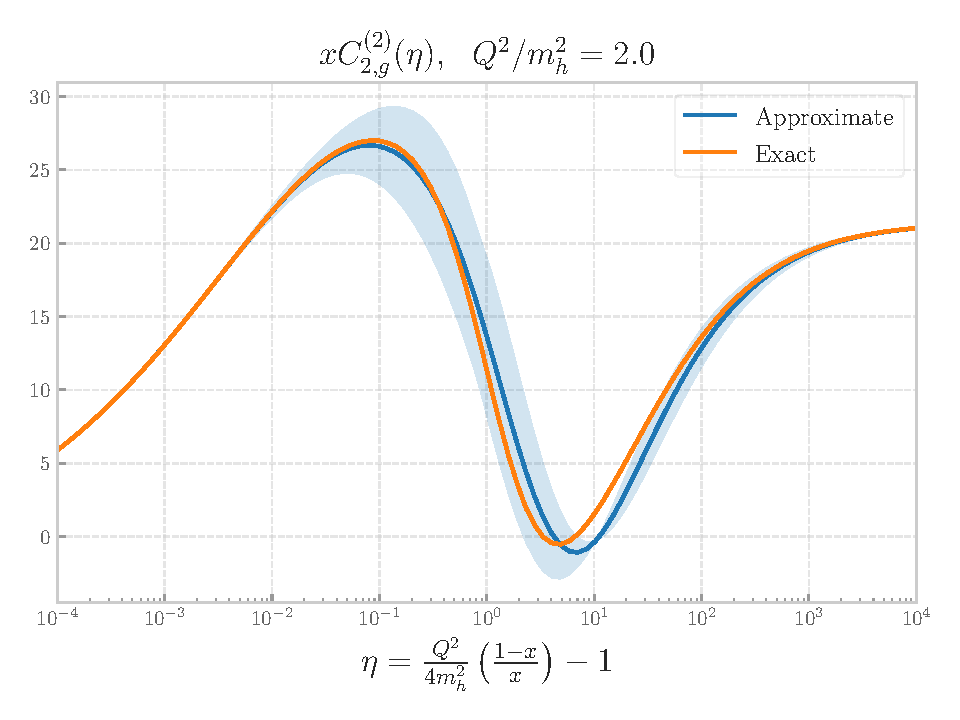
\includegraphics[width=.4\textwidth]{figures/C2g_2_Q2m2_2.0.pdf}
    \caption*{We can validate the procedure at NNLO}
  \end{figure}
\end{frame}


\begin{frame}{DIS variable flavor number scheme}
  \begin{columns}
    \begin{column}{0.59\textwidth}
      \begin{itemize}
        \item In a PDF fit different flavour number schemes are joined in a variable flavour number scheme (VFNS) to ensure reliable results from $Q^2\sim m_h^2$ up to $Q^2\gg m_h^2$
        \item The matching conditions encoding the transition between schemes have almost completely been computed up to N3LO
        \item The VFNS used in NNPDF is the FONLL scheme below
        \item Extended up to N3LO
      \end{itemize}
    \end{column}
    \begin{column}{0.39\textwidth}
      \vspace*{-2em}
      \begin{figure}[!t]
        \centering
        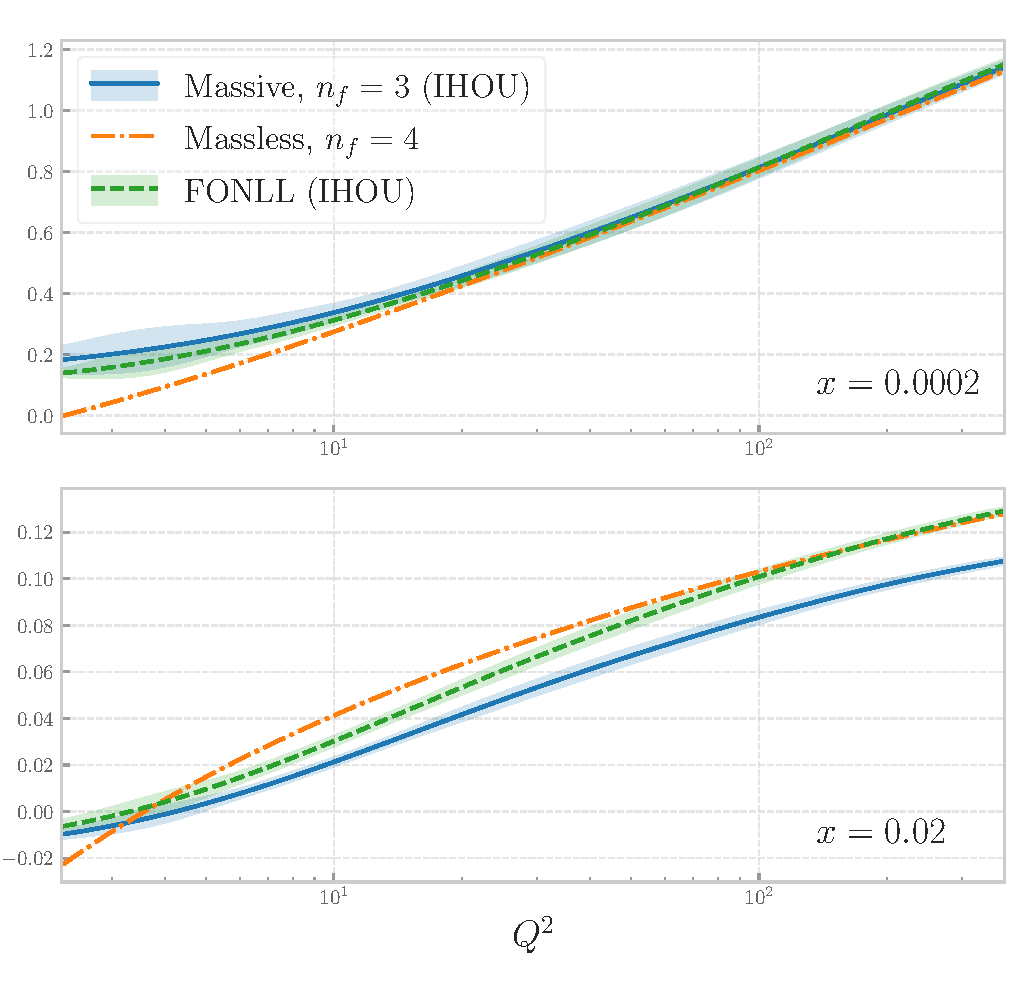
\includegraphics[width=0.89\textwidth]{figures/F2_charm_n3lo.pdf}
        \caption*{$F_2^{(c)}$}
      \end{figure}
    \end{column}
  \end{columns}

  \vspace*{1em}
  \begin{equation*}
    F_\mathrm{FONLL}(Q^2,m_c) =F^{(n_f+1)}(Q^2,m_h=0)
    +F^{(n_f)}(Q^2,m_c)-\lim_{m_c\rightarrow 0}F^{(n_f)}(Q^2,m_h)
  \end{equation*}
  % Up to NNLO, FONLL was implemented expressing the terms in the r.h.s in terms of $\alpha_s$ and PDFs defined in the massless scheme

  % FONLL is now implemented at ``observable level'' with simultaneous PDFs in different flavour number schemes, made possible thanks to the new \texttt{EKO} evolution code and \texttt{yadism} DIS library


\end{frame}




\begin{frame}{DIS structure functions}
  \begin{figure}[!t]
    \centering
    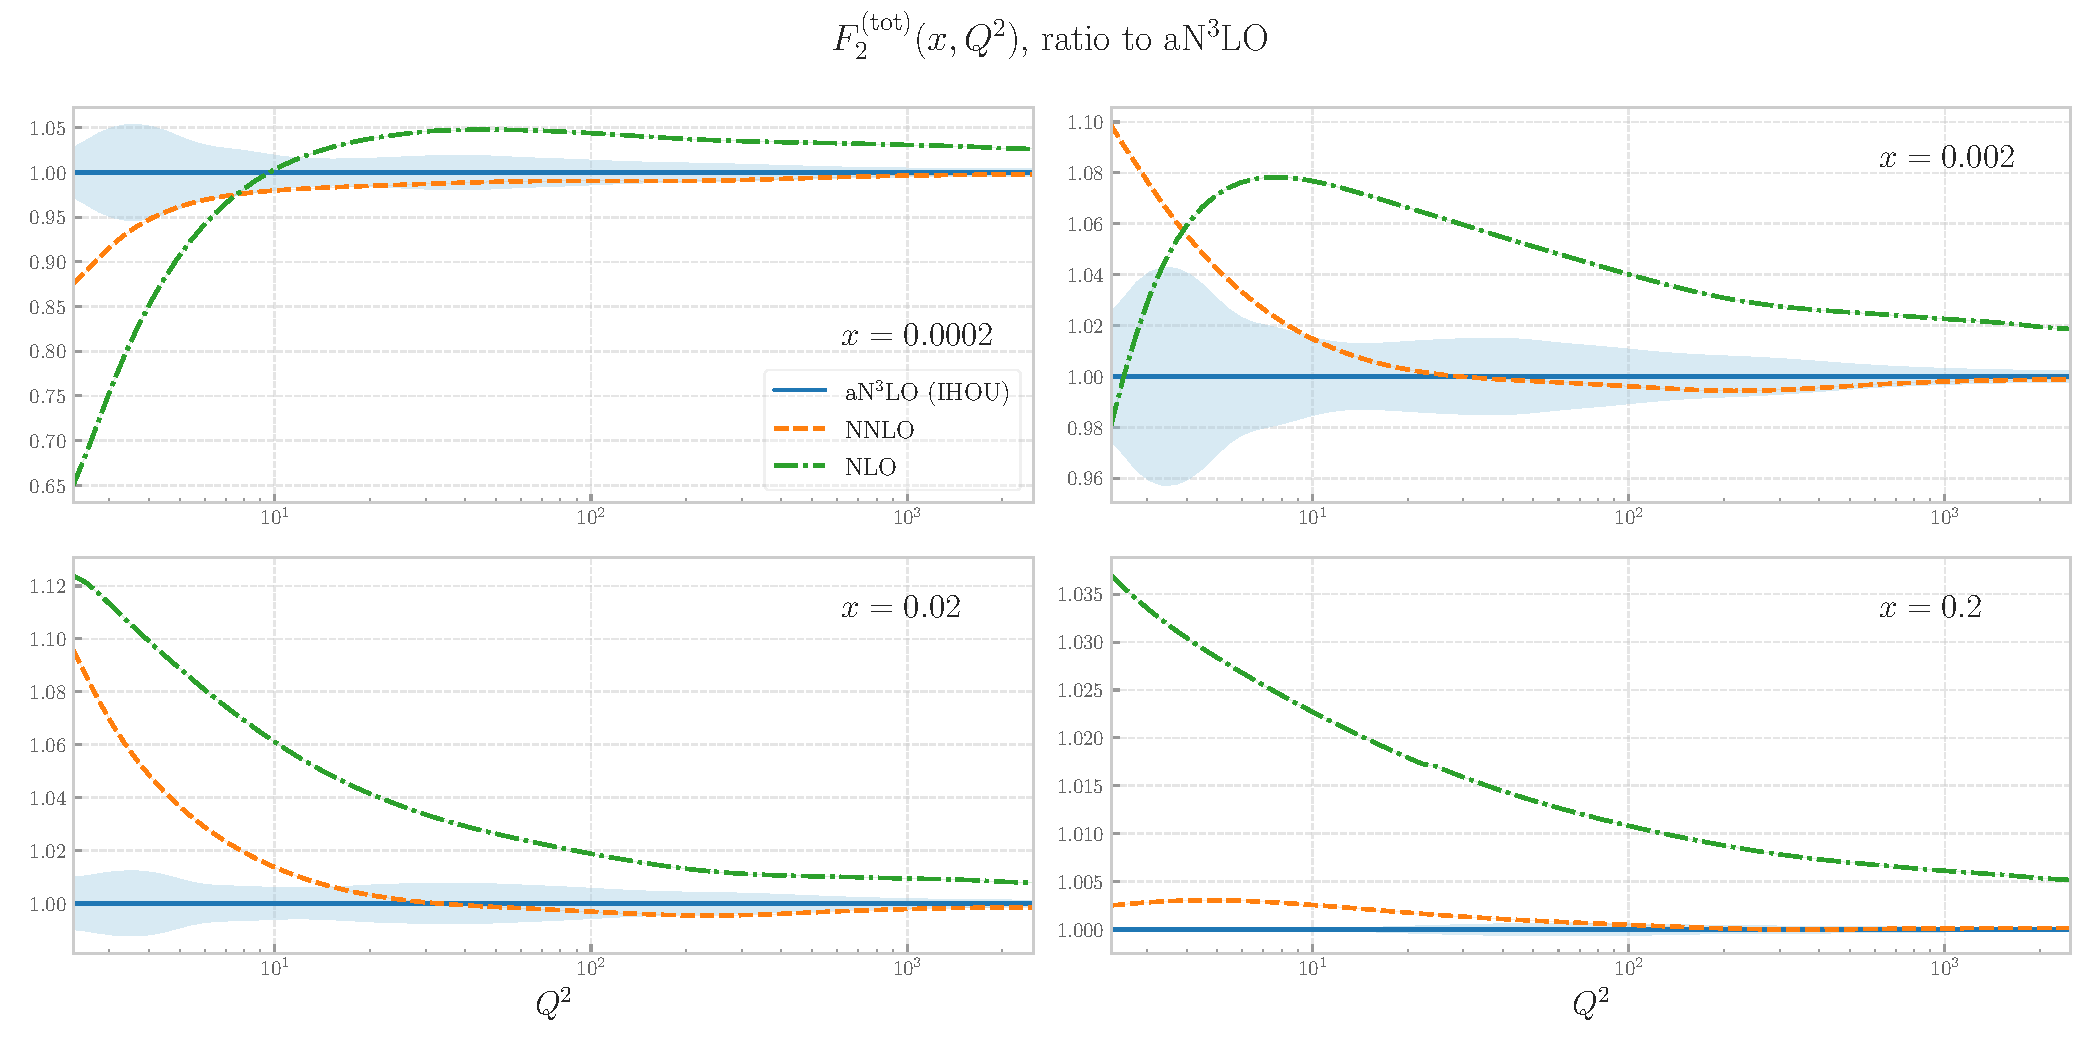
\includegraphics[width=0.75\textwidth]{figures/F2_total.pdf}
  \end{figure}
  \begin{itemize}
    \item unc is IHOU of the massive coefficient functions
    \item N3LO corrections are significant at low-$Q$
  \end{itemize}
\end{frame}


\begin{frame}{Hadronic processes}
  \begin{itemize}
    \item Corrections to collider DY and $W$ production can be included through k-factors
    \item N3LO effects around 1 to 2\%
    \item For many processes N3LO corrections are not available, for those we introduce MHOU
  \end{itemize}
  \begin{figure}[!t]
    \centering
    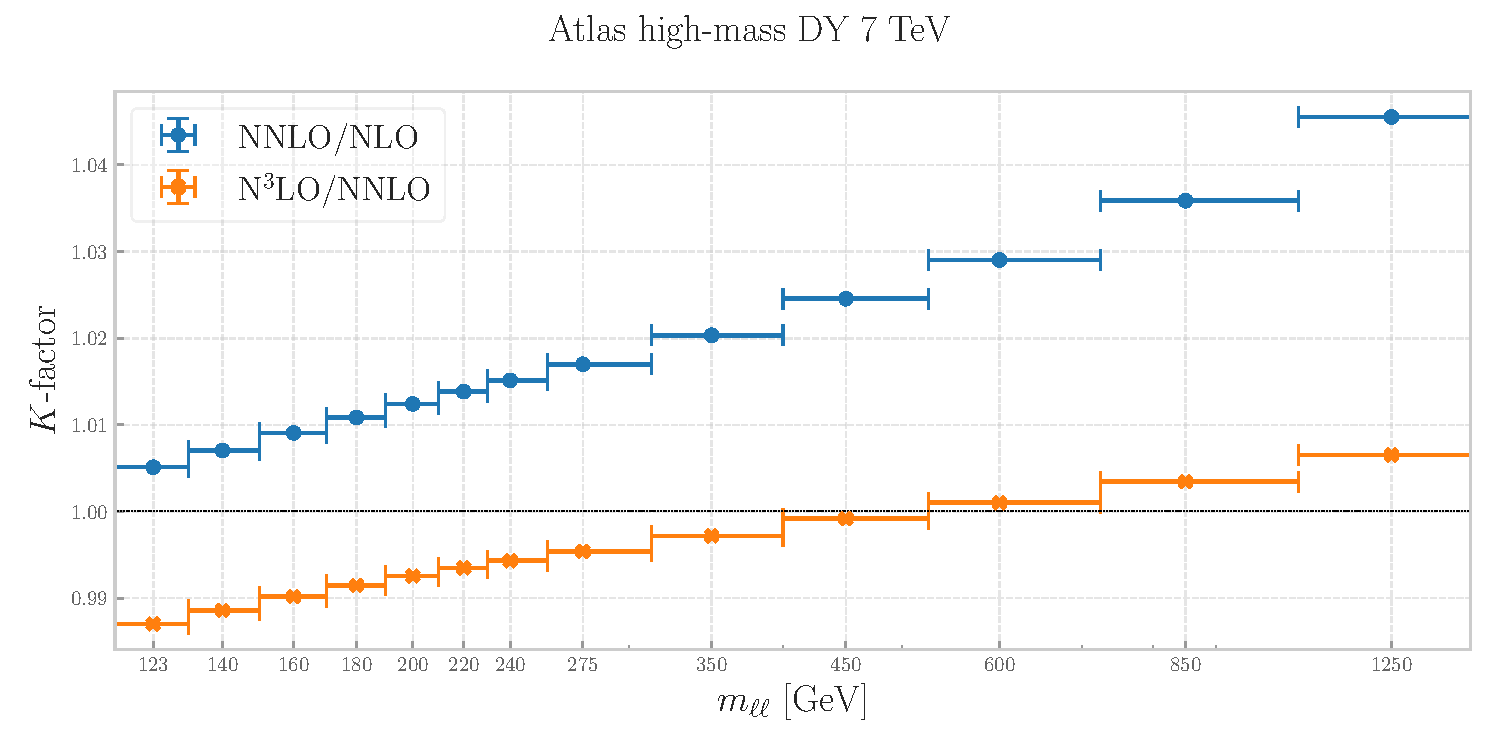
\includegraphics[width=.80\textwidth]{figures/kfactor_ATLASZHIGHMASS49FB.pdf}
  \end{figure}
\end{frame}


% ============================================================================
\section{Inclusion of theory uncertainties}

\begin{frame}{Theory errors from scale variations}
  \begin{itemize}
    \item Missing higher order uncertainties are estimated through variations of the nonphysical factorization ($\mu_f$) and renormalization ($\mu_r$) scales
    \item $\mu_r$ and $\mu_f$ are varied sumultaneously following the 7-point prescription
  \end{itemize}
  \begin{figure}
    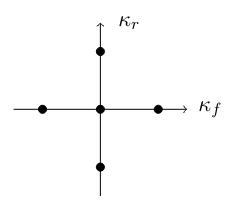
\includegraphics[width=.2\textwidth]{figures/5point.png}
    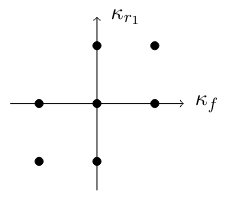
\includegraphics[width=.2\textwidth]{figures/7point.png}
    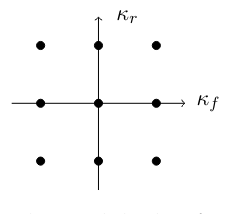
\includegraphics[width=.2\textwidth]{figures/9point.png}
    \caption*{5,7,9 point prescription}
  \end{figure}
  \begin{itemize}
    \item A single factorization scale correlates all points
    \item A renormalization scale per process
  \end{itemize}
\end{frame}

\begin{frame}{Missing higher order uncertainties covmat}

  $P(T|D) \propto \exp\left[-\frac{1}{2}\left(T-D\right)C_\mathrm{exp}^{-1}\left(T-D\right)\right]$
  \begin{itemize}
    \item include theory covmat $C_\mathrm{MHOU}$ at same footing as exp covmat $C_\mathrm{exp}$: $C_\mathrm{exp}\rightarrow C_\mathrm{exp}+C_\mathrm{MHOU}$
  \end{itemize}
  $$C_{\mathrm{MHOU},ij} = n_{m}\sum_{V_{m}}\left(T_{i}(\rho_f, \rho_r) - T_{i}(0, 0)\right)\left(T_{j}(\rho_f, \rho_r) - T_{j}(0, 0)\right)$$

  Can we validate the faithfulness of these uncertainties on the unknown order?

\end{frame}


\begin{frame}{Missing higher order uncertainties covmat}
  Validate the MHOU procedure by testing the NLO MHOU covmat
  \begin{figure}[!t]
    \centering
      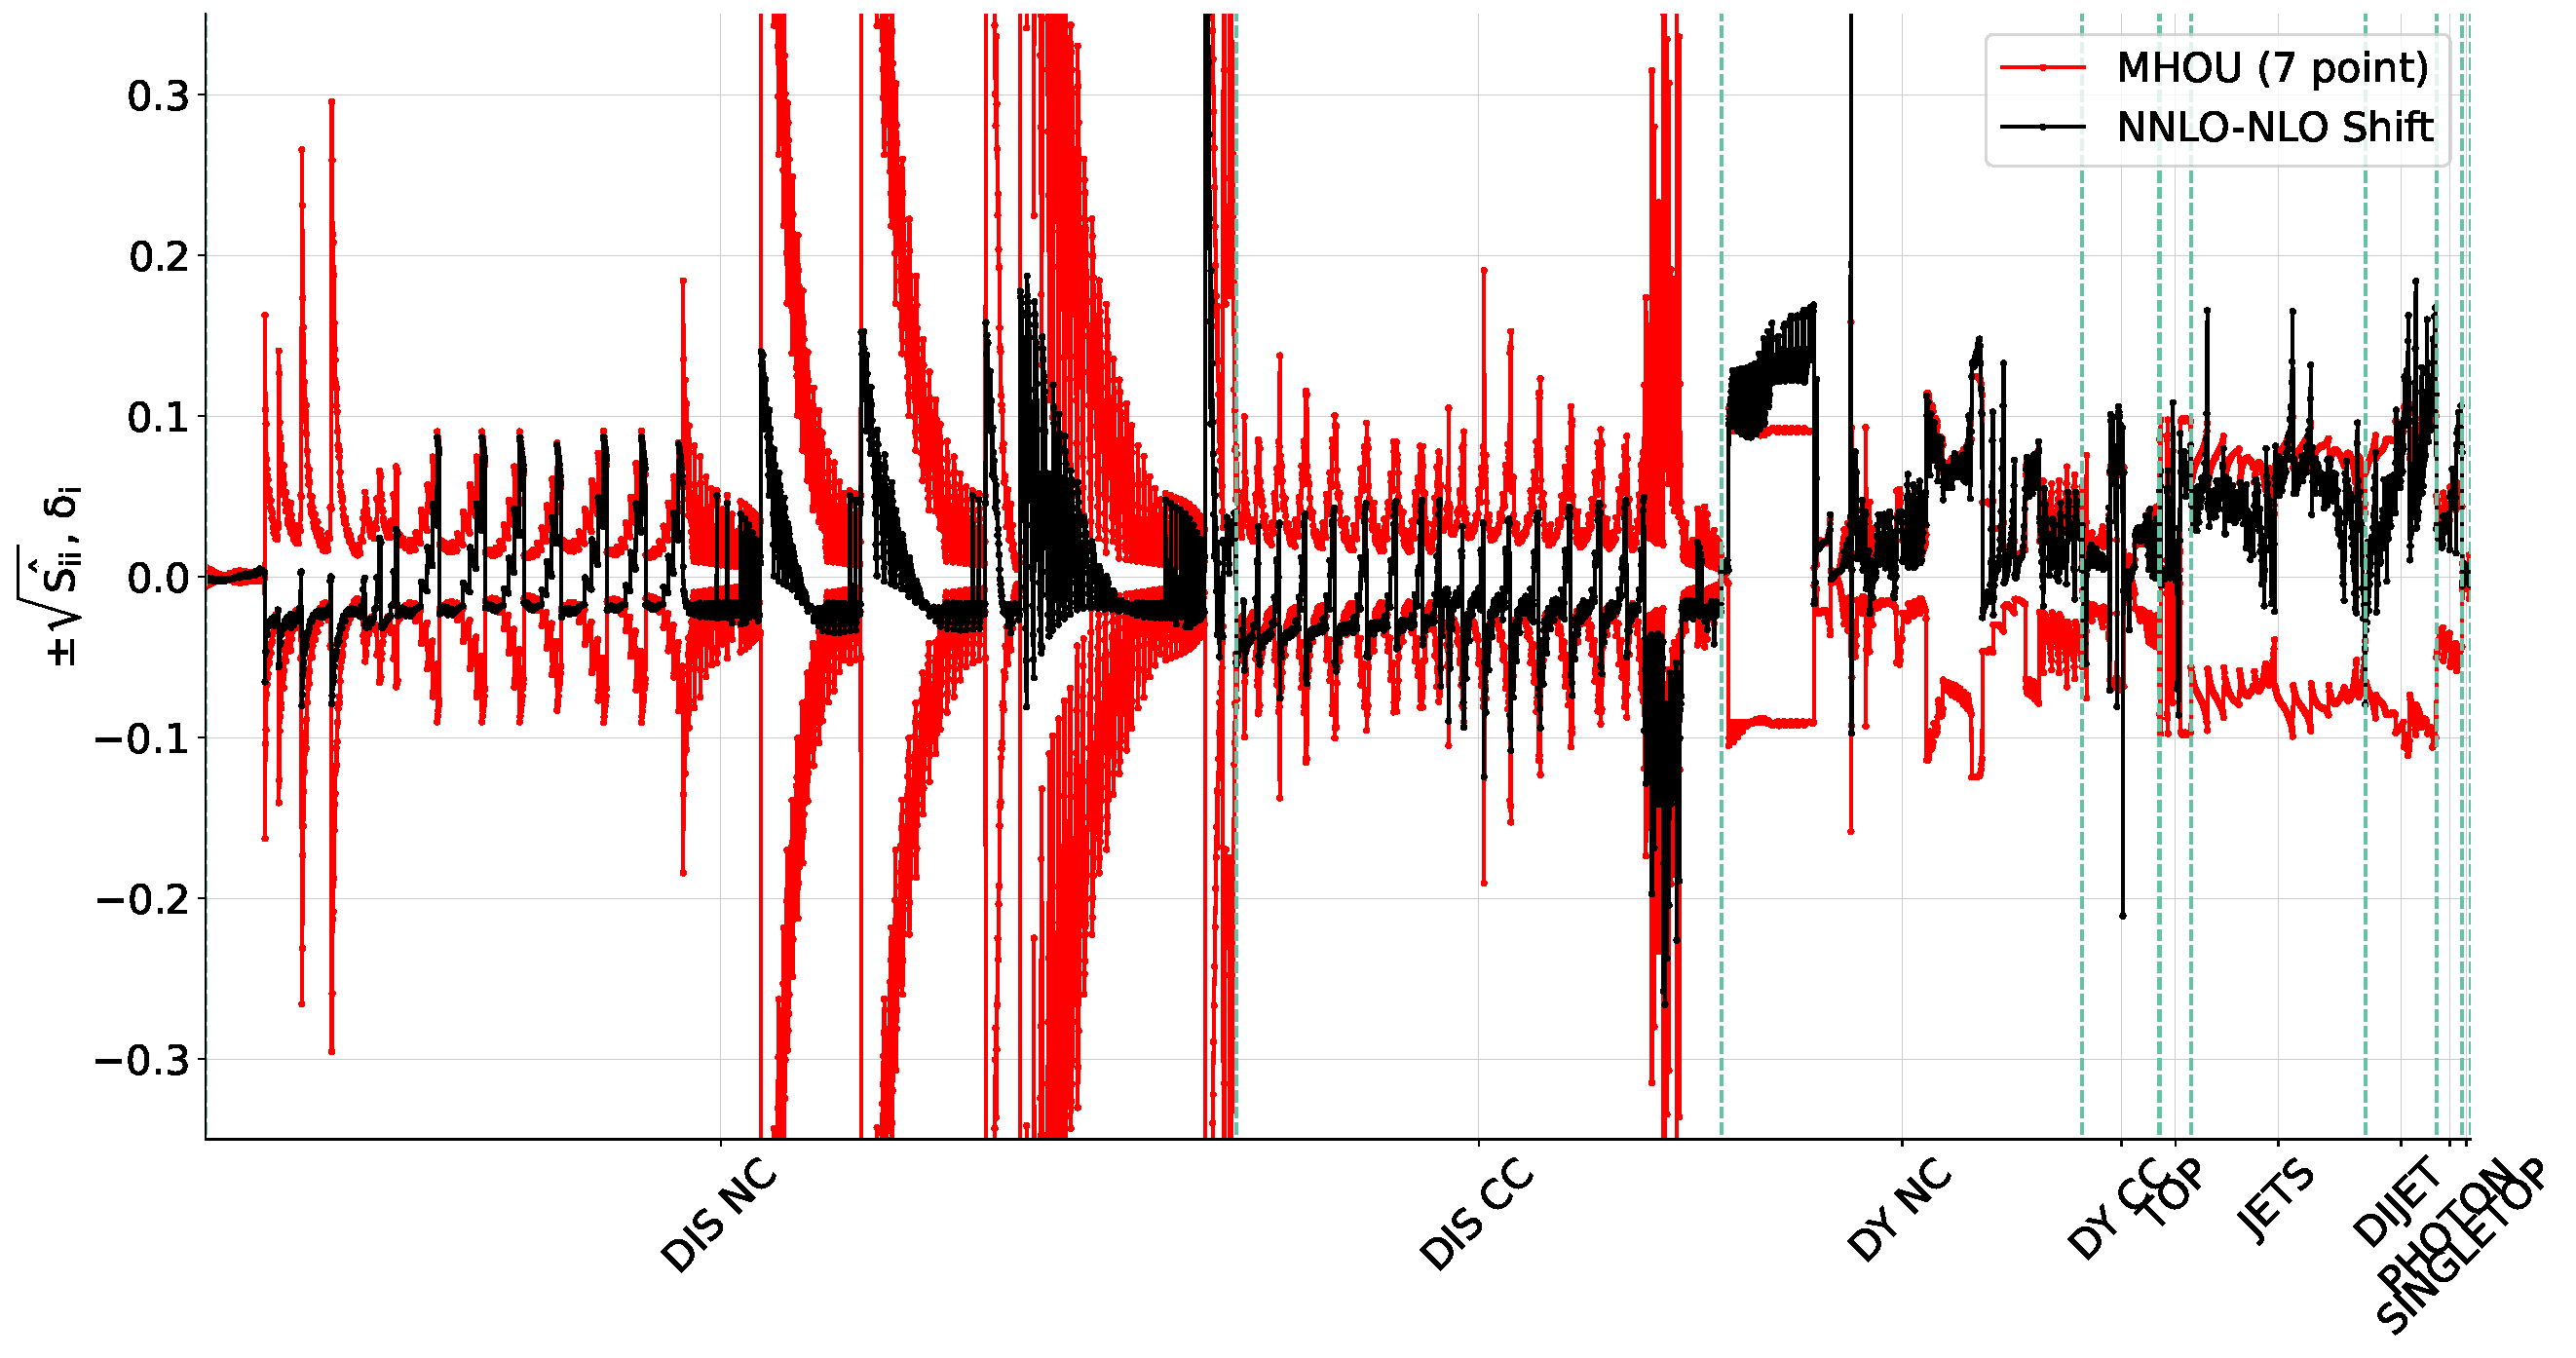
\includegraphics[width=0.6\textwidth]{figures/shift_validation.pdf}
  \end{figure}
\end{frame}

\begin{frame}{Incomplete higher order uncertainties covmat}
  \begin{itemize}
    \item We construct an IHOU matrix following a similar approach
    \item IHOU are independent of MHOU so the uncertainties are added in quadrature
    $$C = C_\mathrm{exp}+C_\mathrm{MHOU}+C_\mathrm{IHOU}$$
  \end{itemize}
  \begin{figure}[!t]
    \centering
    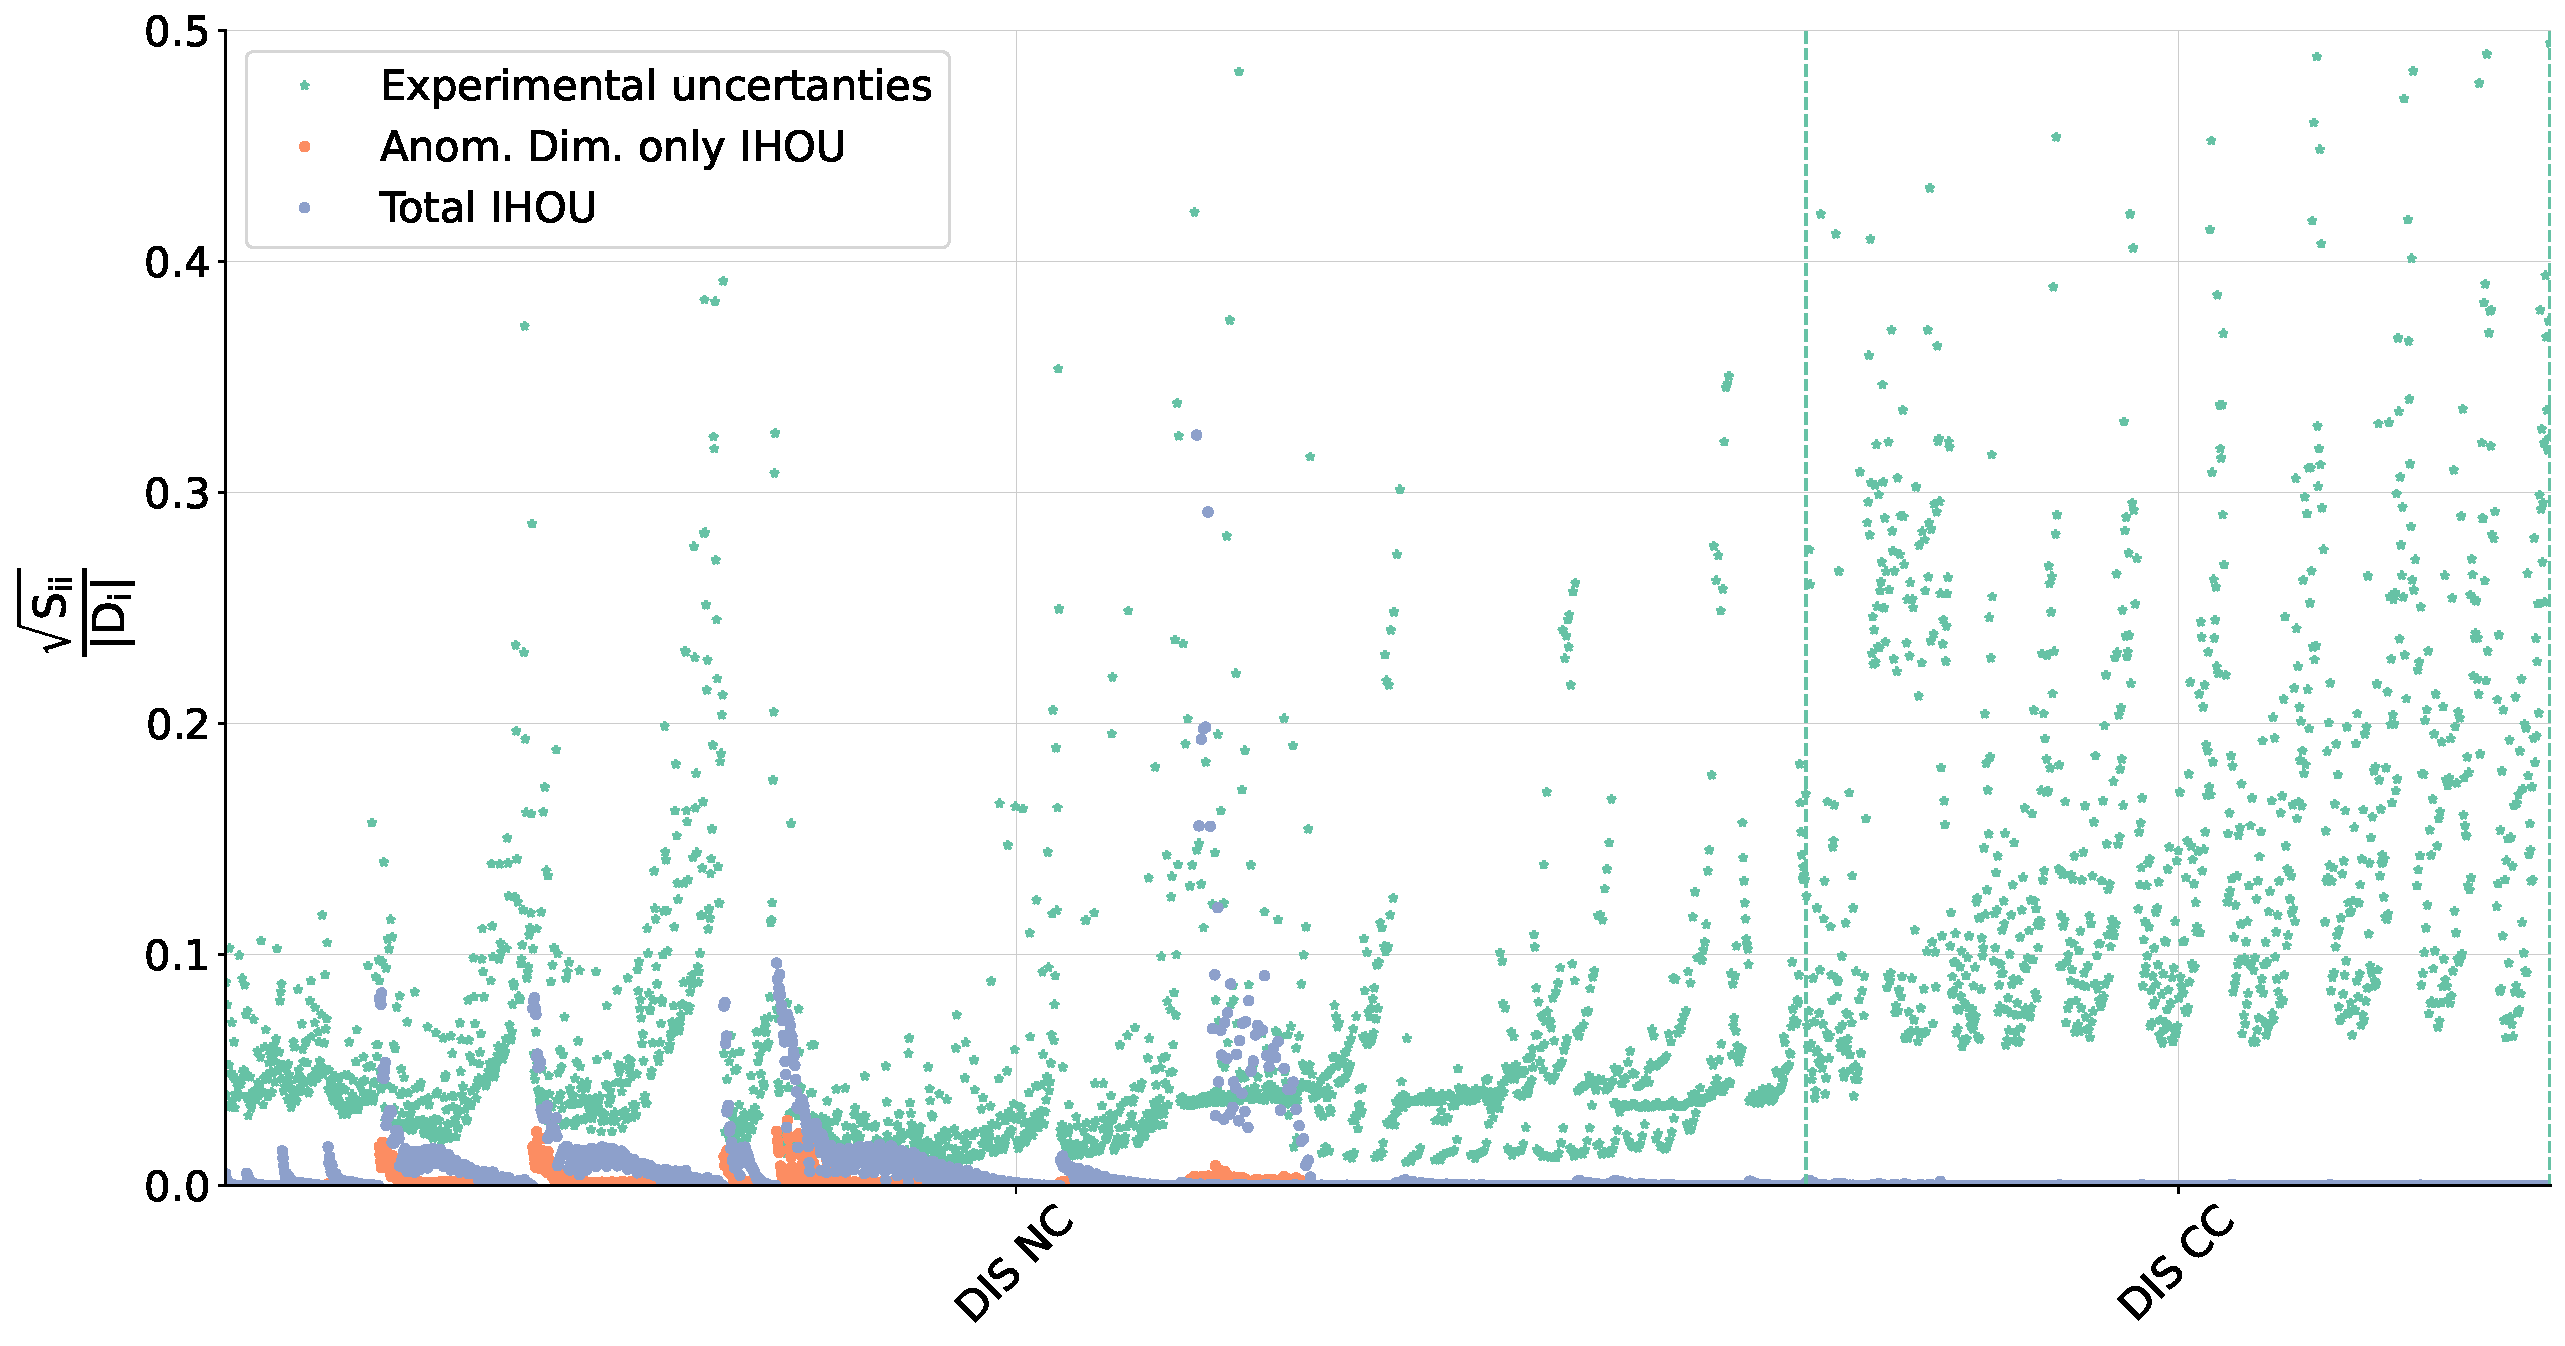
\includegraphics[width=.48\textwidth]{figures/diag_cov_dis_ihou.pdf}
    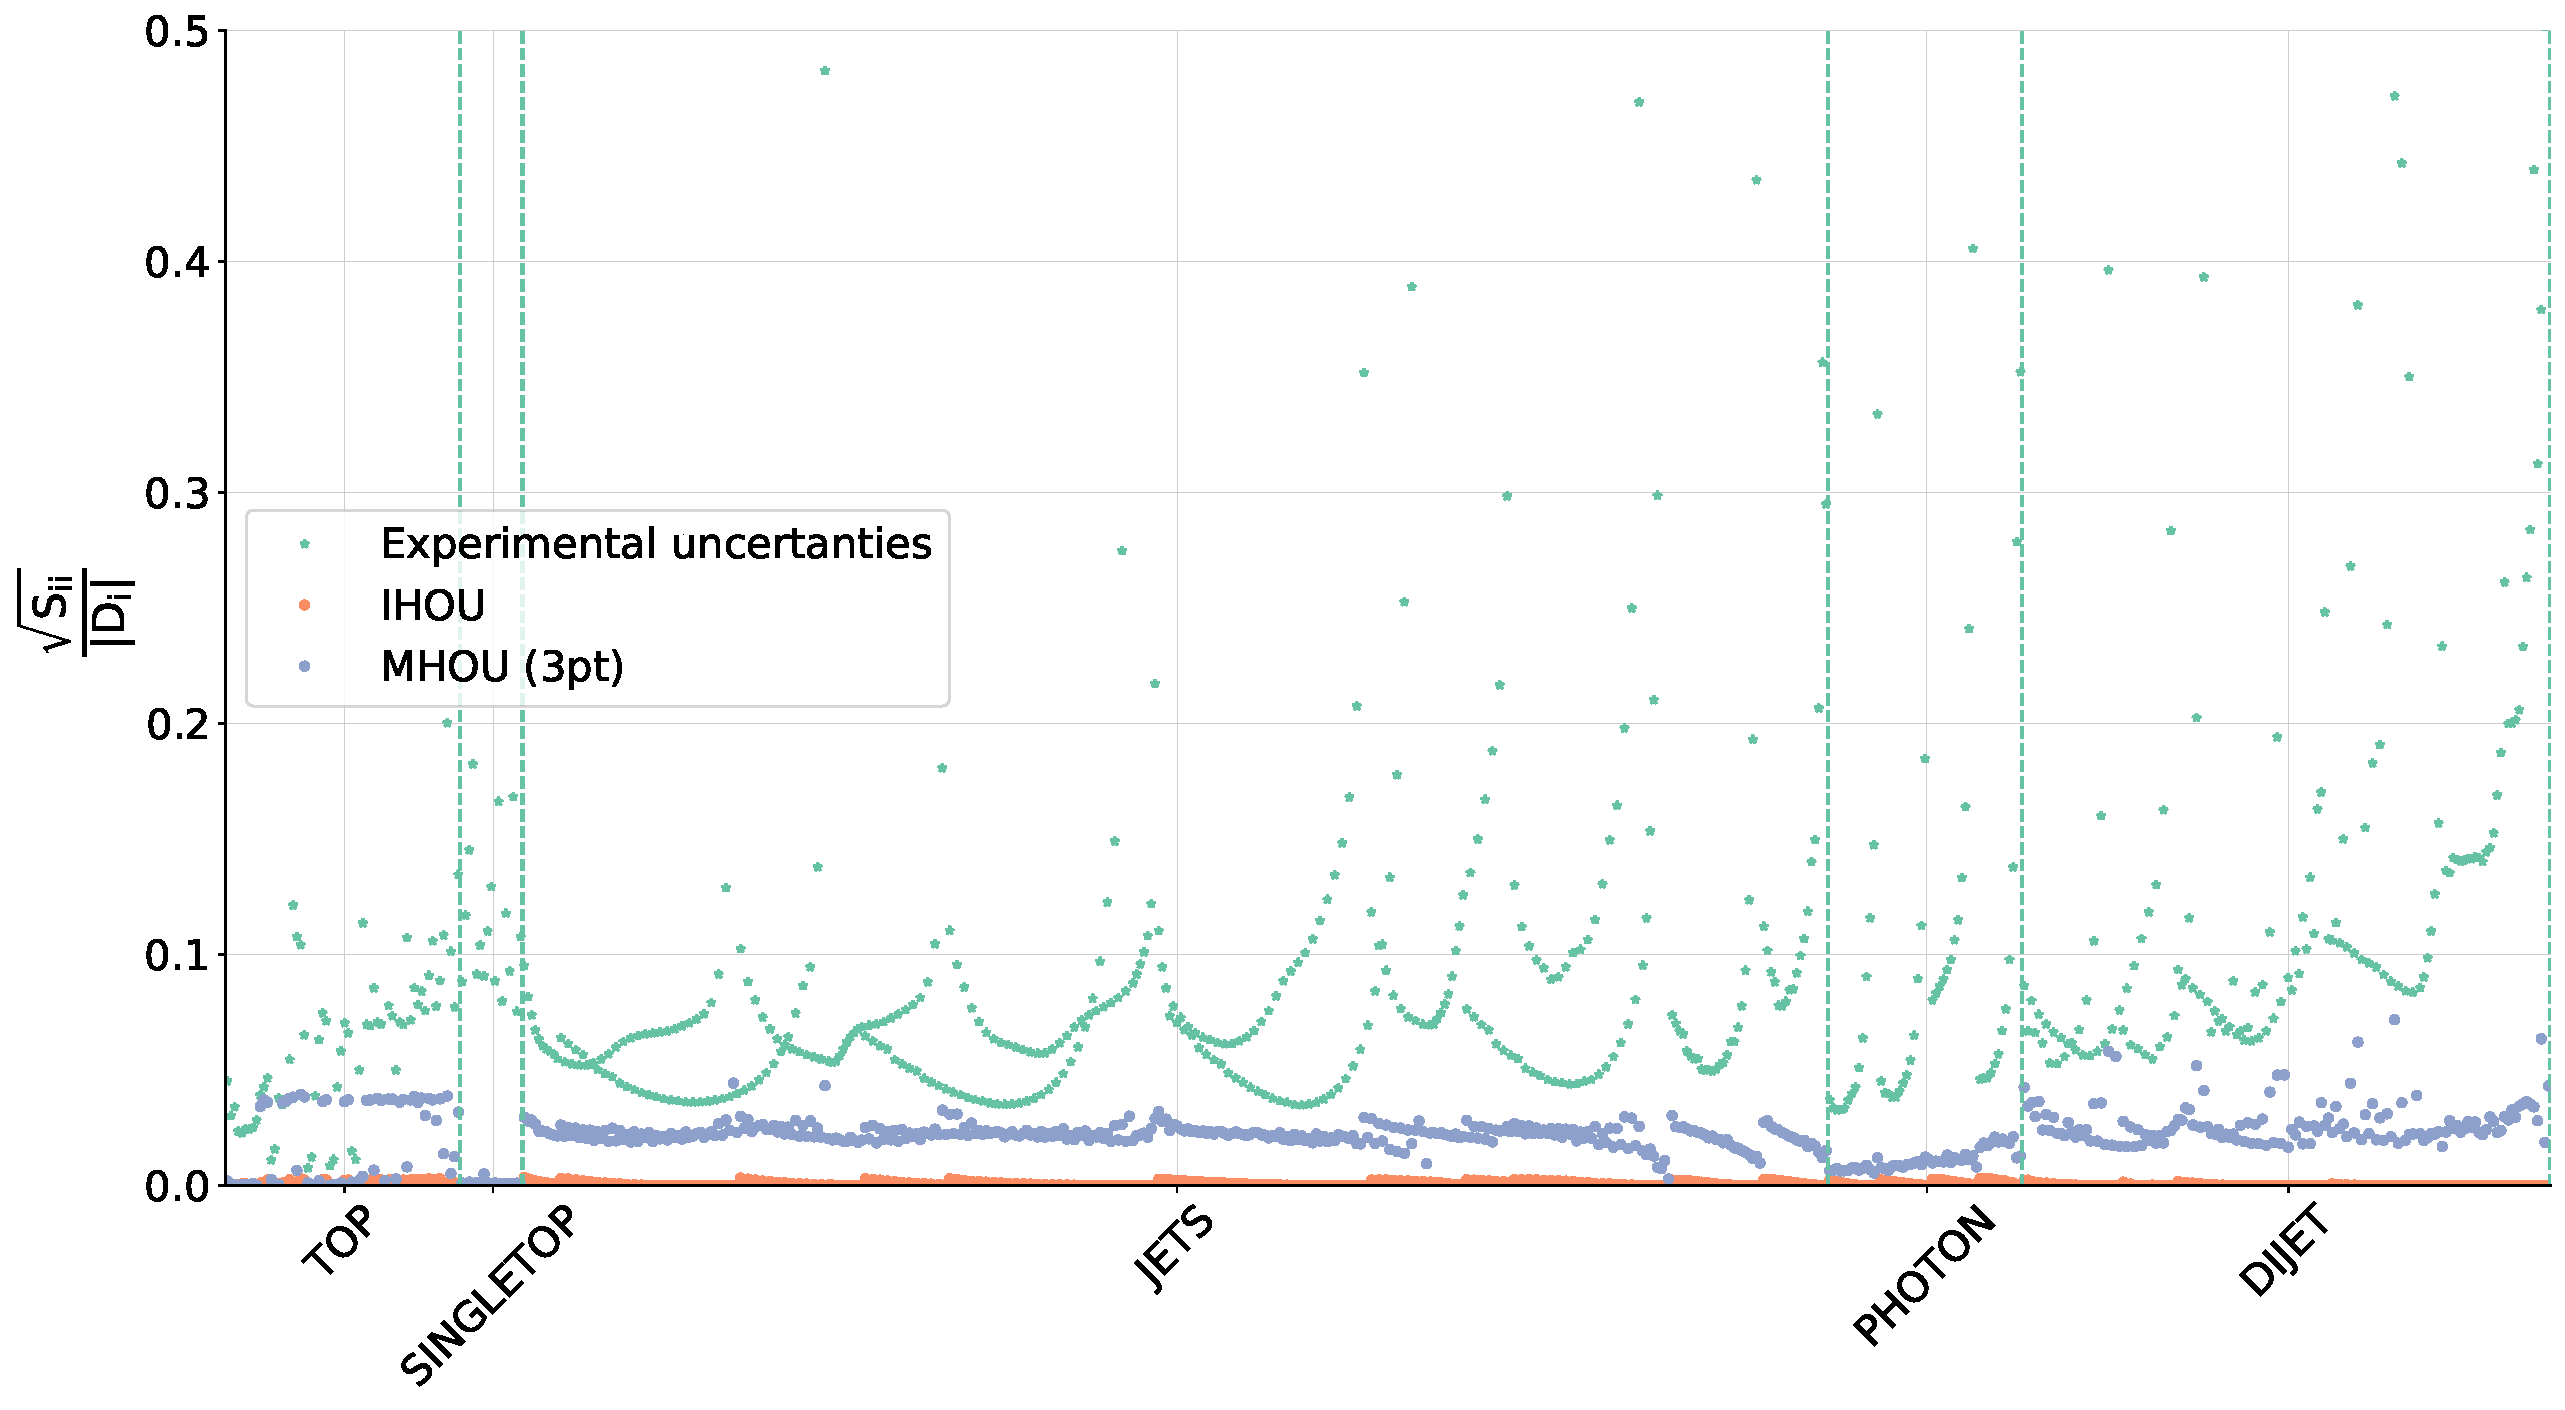
\includegraphics[width=.48\textwidth]{figures/diag_cov_jets_top_ihou_3pt_mhou.pdf}
    \caption*{Fraction of IHOU due to anomalous dimension in DIS $\quad$ MHOU compared to IHOU in hadronic processes}
  \end{figure}
\end{frame}

\begin{frame}{Magnitude of theory uncertainties}
% show that for certain processes th unc is of same size as exp unc.
\end{frame}

% ============================================================================
\section{Results}

\begin{frame}{Fit quality}
  \begin{figure}[!t]
    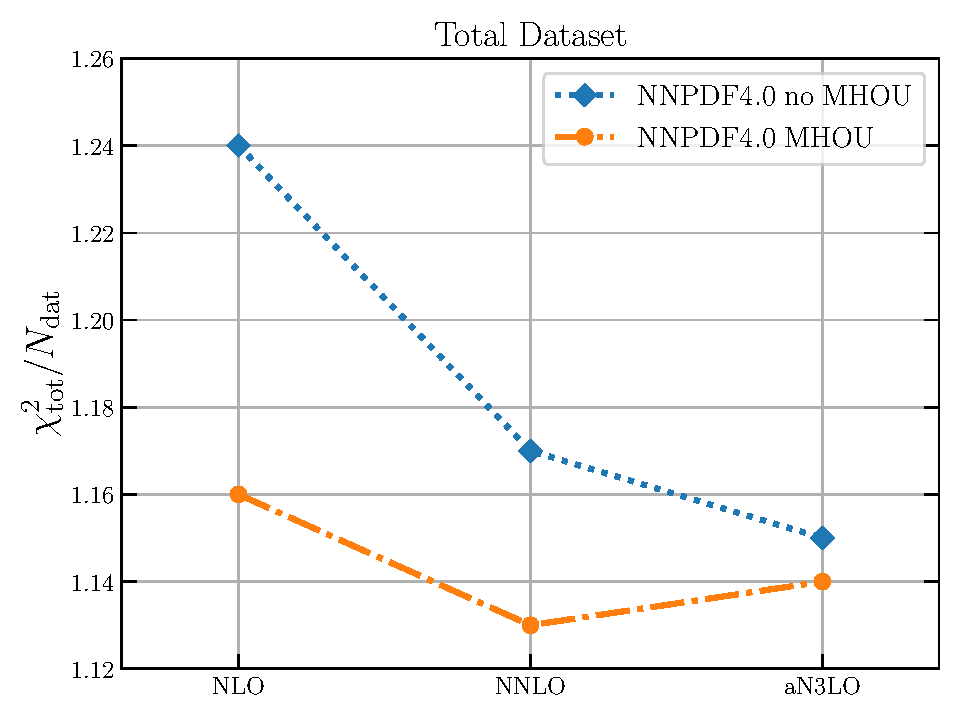
\includegraphics[width=.4\textwidth]{figures/chi2_n3lo_summary.pdf}
  \end{figure}
  \begin{itemize}
    \item Without MHOUs the $\chi^2$ improves with the perturbative accuracy
    \item With MHOUs the $\chi^2$ stabilizes significantly
    \item At N3LO MHOUs have a small impact
  \end{itemize}
\end{frame}

\begin{frame}{Perturbative convergence}
  \begin{figure}[!t]
    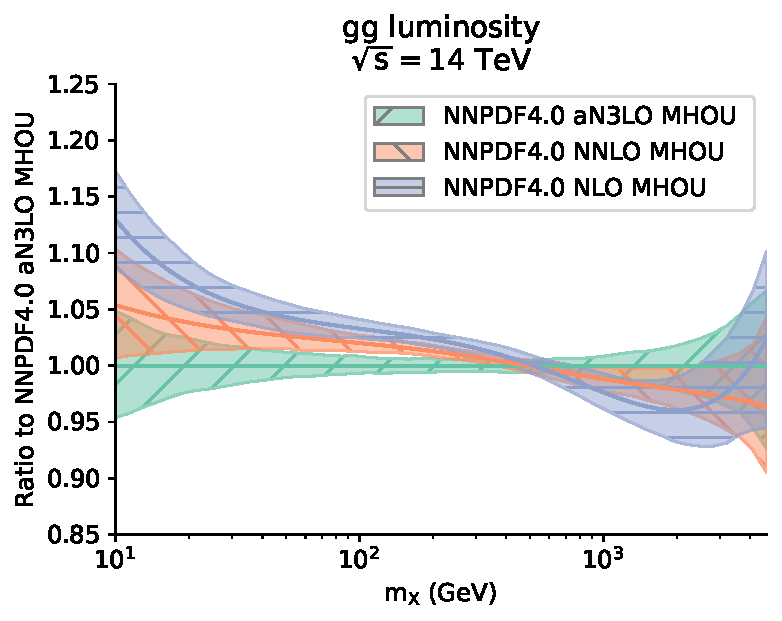
\includegraphics[width=.4\textwidth]{figures/gg_plot_lumi1d_convergence.pdf}
    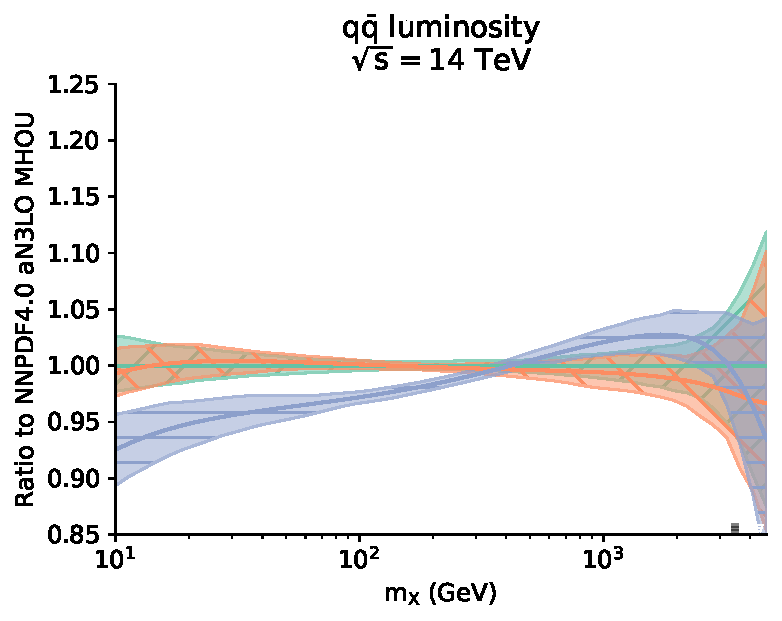
\includegraphics[width=.4\textwidth]{figures/qqbar_plot_lumi1d_convergence.pdf}
  \end{figure}
  \begin{itemize}
    \item Good perturbative convergence
    \item Moderate impact of N3LO corrections, especially for the quark luminosities
    \item $\sim2\%$ suppression of $gg$ luminosity around the Higgs mass
  \end{itemize}
\end{frame}


\begin{frame}{Impact of MHOUs at N3LO}
  \begin{figure}[!t]
    \centering
    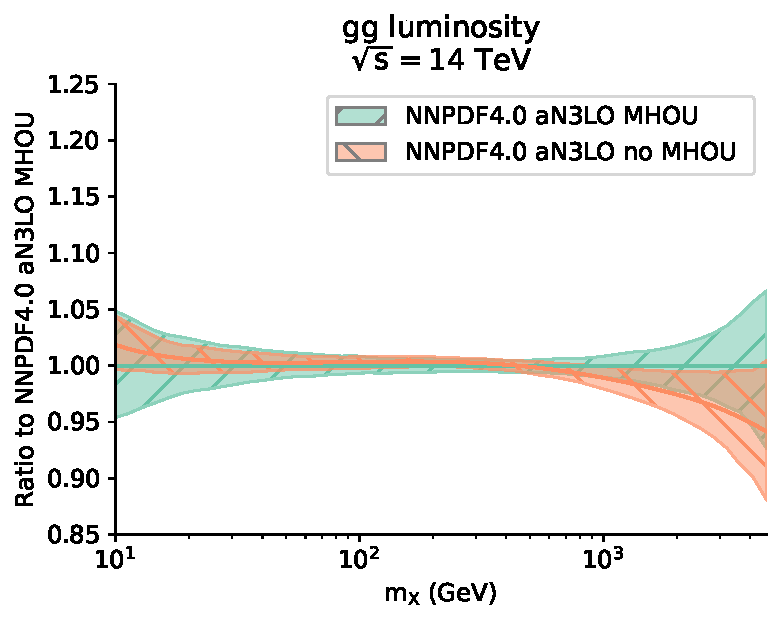
\includegraphics[width=0.45\textwidth]{figures/gg_plot_lumi1d.pdf}
    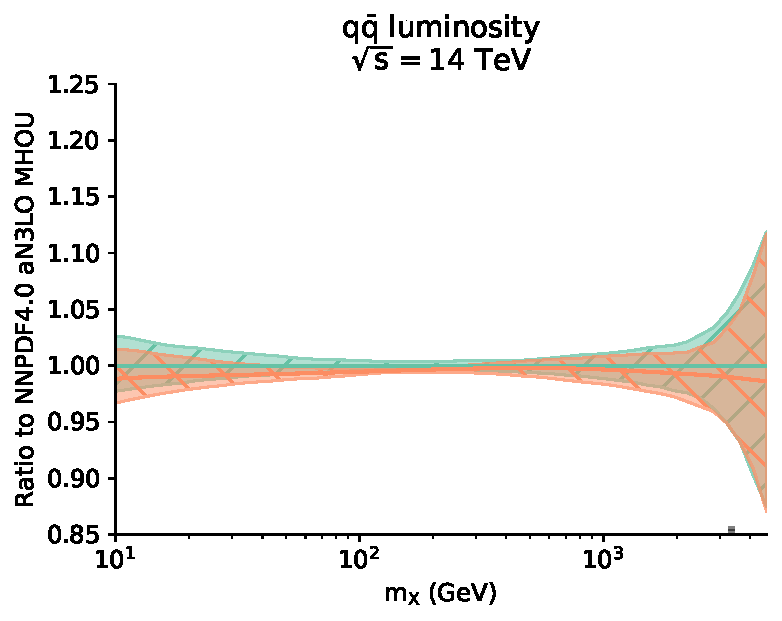
\includegraphics[width=0.45\textwidth]{figures/qqbar_plot_lumi1d.pdf}
  \end{figure}
  \begin{itemize}
    \item Non-negligible impact of MHOUs even at N3LO
    \item[$\Rightarrow$] reason to include exact N3LO calculations for hadronic processes
  \end{itemize}
\end{frame}


\begin{frame}{Comparison to MSHT20}
  \begin{figure}[!t]
    \centering
    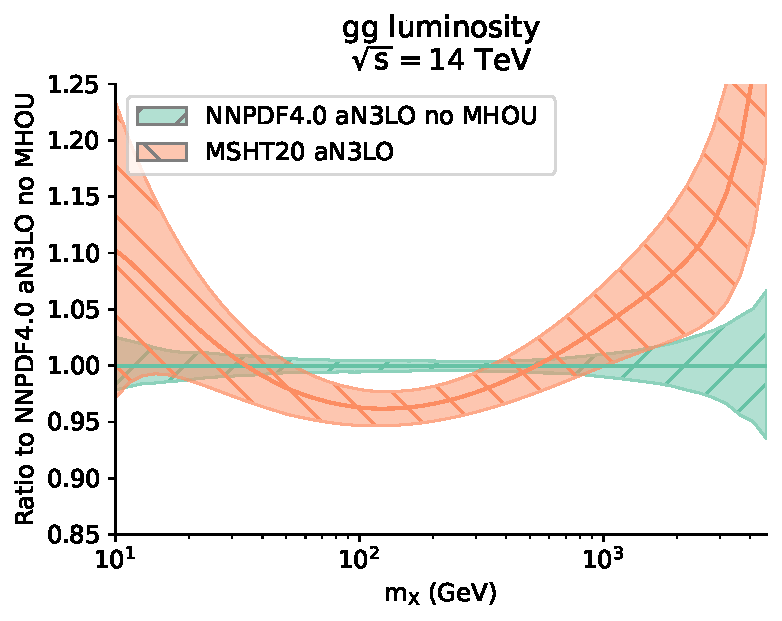
\includegraphics[width=0.45\textwidth]{figures/gg_plot_lumi1d_msht20.pdf}
    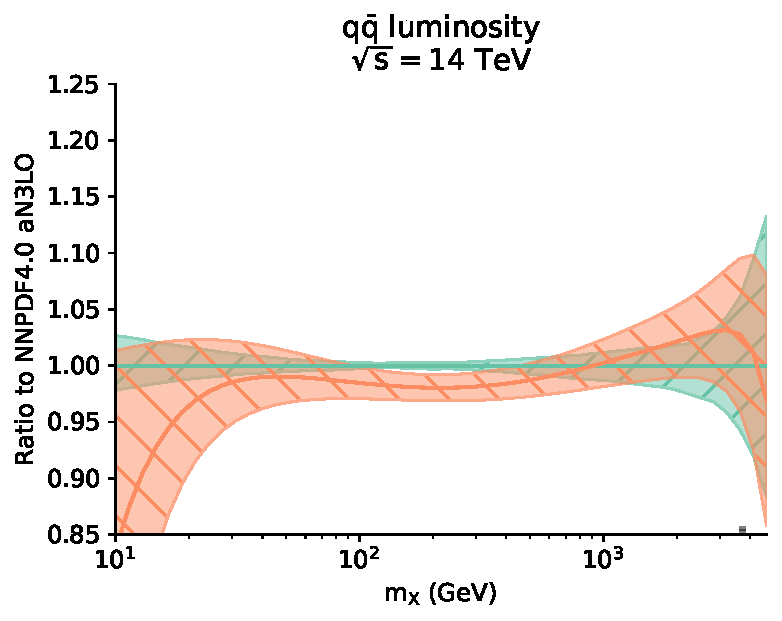
\includegraphics[width=0.45\textwidth]{figures/qqbar_plot_lumi1d_msht20.pdf}
  \end{figure}
  \begin{itemize}
    \item Good agreement with MSHT20 for the quark luminosities
    \item Also for gluon luminosities, except around the Higgs mass and high-mass
    \item Similar data but different methodology (including splitting function parametrization)
  \end{itemize}
\end{frame}


\section{LHC phenomenology}

\begin{frame}{Higgs production}
  \begin{figure}[!t]
    \centering
    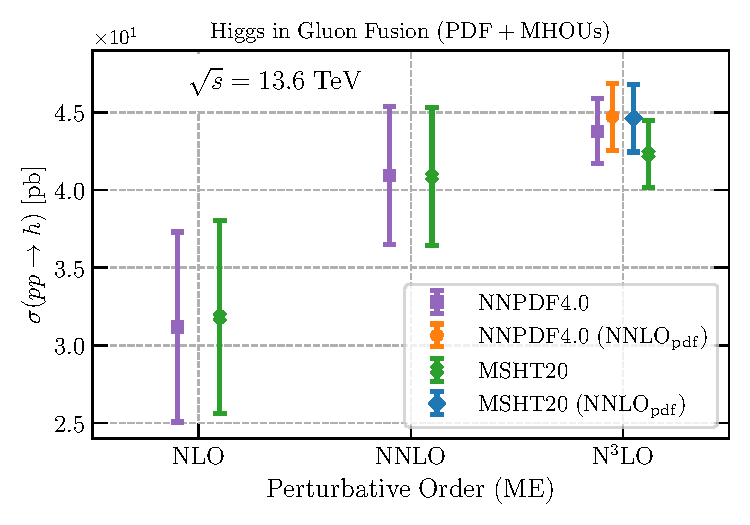
\includegraphics[width=0.49\linewidth]{figures/higgs-ggF-n3lo.pdf}
    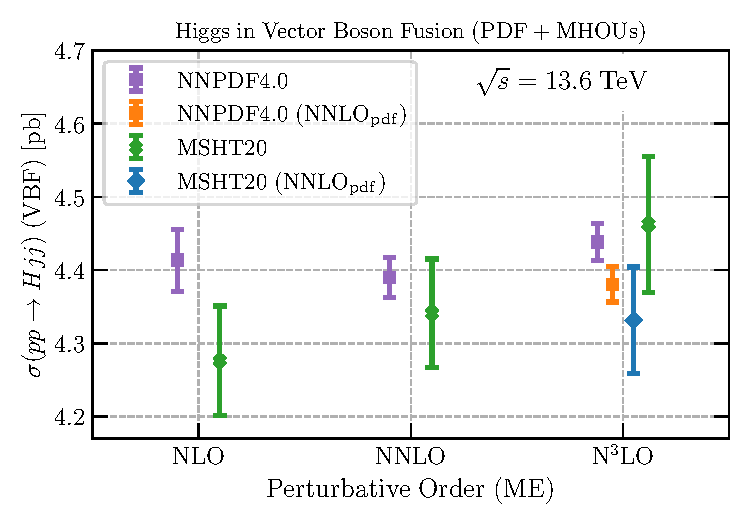
\includegraphics[width=0.49\linewidth]{figures/H_VBF-n3lo.pdf}
  \end{figure}
  \begin{itemize}
    \item Matrix elements for both Higgs in gluon fusiona and VBF available at N3LO
    \item N3LO correction to Higgs in gluon fusion, small suppression compared to NNLO
    \item Higgs in VBF perturbatively stable
  \end{itemize}
\end{frame}


\begin{frame}{Drell-Yan}
  \begin{figure}[!t]
    \centering
    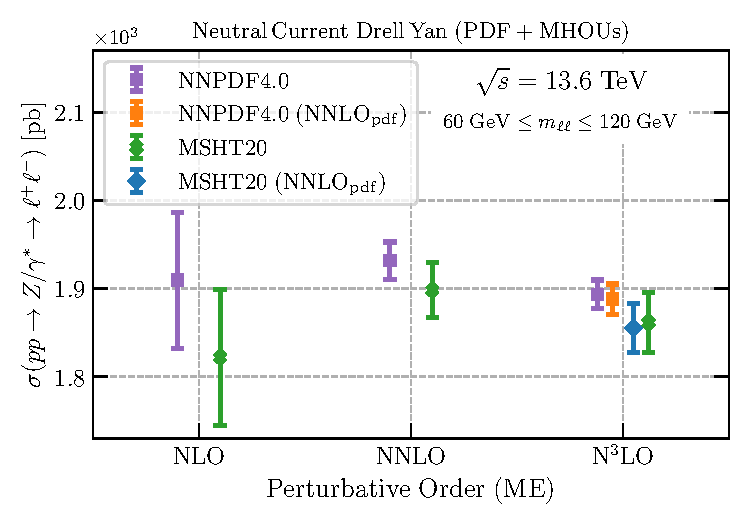
\includegraphics[width=0.49\linewidth]{figures/Z_60_120-n3lo.pdf}
    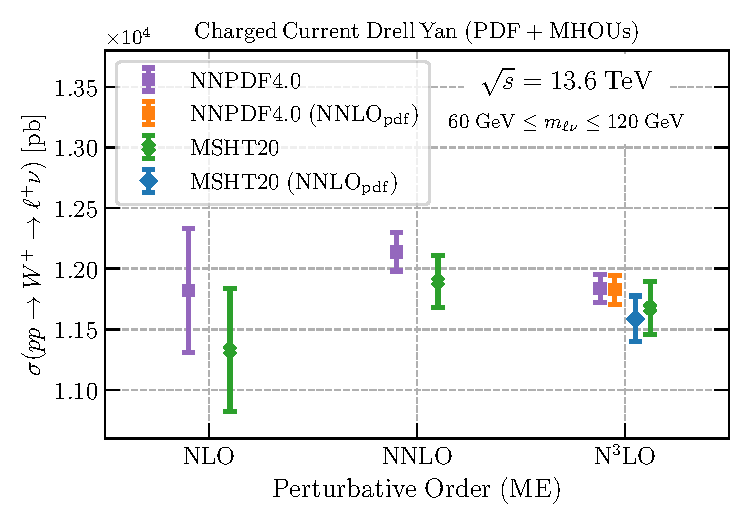
\includegraphics[width=0.49\linewidth]{figures/Wp_60_120-n3lo.pdf}
  \end{figure}
  \begin{itemize}
    \item Good convergence also for quark initiated processes
  \end{itemize}
\end{frame}



\section{Summary and outlook}
\begin{frame}{Summary and outlook}
  \begin{itemize}
    \item N3LO PDFs are a requirement for LHC predictions at 1\% accuracy
    \item All sources of theory uncertainty should be accounted for
    \item NNPDF4.0 aN3LO allows for consistent N3LO calculations. Initial results for Higgs and DY production suggest good perturbative convergence
    \item Ongoing effort to benchmark these results with other groups
    \item Work towards combining N3LO, MHOU and QED is ongoing
  \end{itemize}
\end{frame}


\end{document}
